\documentclass[11pt, a4paper]{article}

% --- Packages ---
\usepackage[margin=1in]{geometry}
\usepackage{amsmath, amssymb, amsthm}
\usepackage{mathpazo}
\usepackage{setspace}
\usepackage{hyperref}
\usepackage{natbib}
\usepackage{titlesec}
\usepackage{color}
\usepackage{booktabs}
\usepackage{graphicx}
\usepackage[dvipsnames]{xcolor}
\usepackage{enumitem}
\usepackage{tikz}
\usetikzlibrary{arrows.meta, decorations.markings, patterns, calc, positioning}
\usepackage{multirow}
\usepackage{float}
\usepackage{caption}
\usepackage{subcaption}
\usepackage{adjustbox}
\usepackage{threeparttable}
\usepackage{dcolumn}
\newcolumntype{d}[0]{D{.}{.}{-1}}
\usepackage{pdflscape}
\usepackage{appendix}

\hypersetup{colorlinks=true, linkcolor=blue, citecolor=blue, urlcolor=blue}
\bibliographystyle{aer}

\onehalfspacing

\title{Creative Destruction in the Market for Intelligence:\\ Demand Reallocation When New LLMs Enter}
\author{Auto-Research Agent\thanks{This paper was produced by an autonomous AI research agent as a methodological demonstration. All analysis uses publicly available data from OpenRouter. Correspondence: N/A.}}
\date{March 2026}

\begin{document}
\maketitle

% === ABSTRACT ===
\begin{abstract}
\noindent Between December 2025 and March 2026, nearly 400 large language models competed for usage on OpenRouter, a major API aggregation platform serving over one million developers. We study how demand reallocates when new models enter this market, decomposing adjustment into three channels: intra-firm cannibalization, cross-firm displacement, and market expansion. Using a nested logit demand model \`{a} la \citet{berry1994estimating}, we estimate that models within the same firm are substantially closer substitutes than models across firms (nesting parameter $\hat{\sigma} = 0.46$, SE $= 0.04$). A descriptive panel analysis of 385 models over 93 days reveals that creative destruction operates almost exclusively through \emph{within-family upgrades}: when a firm releases a successor in the same model family, the predecessor is associated with approximately 35\% fewer daily requests ($\hat{\beta} = -0.43$, SE $= 0.16$). Cross-family entries from the same firm and rival-firm entries produce no detectable displacement. Alternative nesting structures by capability tier and price tier yield near-perfect within-group substitution ($\hat{\sigma} > 0.99$), confirming that the relevant competitive margin is defined by model characteristics rather than firm identity alone. These patterns are consistent with Schumpeterian creative destruction concentrated along quality ladders, where each generation of a model family replaces the last, while the overall market continues to expand. The absence of cross-firm displacement in the short run---even in a setting with near-zero switching costs---suggests that horizontal differentiation across providers is sufficient to insulate firms from each other's entries during the current rapid-growth phase of the market.

\medskip
\noindent \textbf{JEL Codes}: L13, L86, O33 \\
\textbf{Keywords}: LLM, API market, creative destruction, nested logit, demand substitution, product entry
\end{abstract}

\newpage

% === 1. INTRODUCTION ===
\section{Introduction}

In the first quarter of 2026, a developer choosing a large language model (LLM) for an API-based application faced a remarkable menu: nearly 400 models from 66 providers, spanning a 100-fold range in per-token prices and capabilities from simple text completion to multi-step reasoning and tool use. New models appeared at a rate of six per week. Yet usage remained heavily concentrated---the top ten models captured over 55\% of requests, and the top firm alone accounted for roughly 15\% of daily traffic.

This paper asks a foundational question about competition in this nascent market: when a new model enters, where does its demand come from? We decompose demand reallocation into three channels. \emph{Intra-firm cannibalization} occurs when a new model draws users away from the releasing firm's existing models. \emph{Cross-firm displacement} occurs when rivals lose traffic. \emph{Market expansion} occurs when the new model attracts usage that would not otherwise have occurred on the platform.

The relative magnitude of these channels matters for market structure, innovation incentives, and welfare. If cannibalization dominates, then the ``replacement effect'' of \citet{arrow1962economic} is operative: incumbents internalize the business-stealing effect of their own innovations, potentially dampening the incentive to release new models. Under this scenario, a firm contemplating a new release must weigh the revenue from new adopters against the revenue lost from users who switch away from its existing models. If cross-firm displacement dominates, the market resembles textbook Schumpeterian competition, where entrants destroy incumbent rents, and the incentive to innovate comes from capturing rivals' market share. If market expansion dominates, entry is largely non-rivalrous in the short run---new models grow the pie rather than reallocating slices---and the market is still in its growth phase, where competitive pressure is less intense than the number of competing products might suggest.

Understanding these dynamics also matters for market participants beyond model providers. Application developers building on LLM APIs face the risk that their chosen model will be displaced or deprecated. If displacement is concentrated within product families (model $X$ v2 replacing $X$ v1), then developers primarily need to manage \emph{upgrade risk} within their chosen provider. If cross-firm displacement is substantial, developers face the more complex challenge of \emph{provider risk}---the possibility that their entire provider's model line becomes uncompetitive. The empirical patterns we document have direct implications for the hedging strategies (e.g., multi-model architectures, model-agnostic abstractions) that application developers adopt.

We use daily model-level usage data from OpenRouter, a leading API aggregation platform, covering 385 models from 66 firms over 93 days (December 2025 to March 2026). OpenRouter provides a unified endpoint through which developers can route requests to models from OpenAI, Google, Anthropic, Meta, Mistral, DeepSeek, and dozens of other providers. The platform's architecture---where switching between models requires changing a single parameter in an API call---makes it an ideal setting to study demand substitution: switching costs are near zero, and we observe the universe of choices at daily frequency.

Our empirical approach has two components. First, we estimate a nested logit demand model \citep{berry1994estimating, mcfadden1978modelling} in which models are grouped by firm. The key parameter $\sigma$ measures the correlation of unobserved preferences within nests: $\sigma$ near one implies that consumers view same-firm models as near-perfect substitutes, while $\sigma$ near zero implies that firm identity is irrelevant to substitution. Our OLS estimate is $\hat{\sigma} = 0.46$ (SE $= 0.04$), indicating that within-firm models are moderately closer substitutes than cross-firm models, but far from perfect substitutes. This estimate is stable across a wide range of outside-option assumptions and robust to the inclusion of model characteristics; an \citet{oster2019unobservable} stability analysis yields $\delta = 155$, indicating that unobservables would need to be over 150 times as important as observables to drive $\sigma$ to zero.

Second, we conduct a descriptive panel analysis of demand changes around model entry events. The aggregate same-firm entry indicator is economically small and statistically indistinguishable from zero ($\hat{\beta} = -0.0004$, SE $= 0.004$). This null result, however, masks sharp heterogeneity. Decomposing same-firm entries into \emph{within-family upgrades} (e.g., GPT-4o replacing GPT-4, Claude 3.5 Sonnet replacing Claude 3 Sonnet) and \emph{different-family entries}, we find that the entire displacement effect is concentrated in upgrades: the within-family coefficient is $-0.43$ (SE $= 0.16$, $p < 0.01$), while the different-family coefficient is essentially zero. Cross-firm entry effects are also negligible. Event study plots corroborate these patterns and show no evidence of differential pre-trends in the days before same-firm entry.

Three additional findings round out the picture. First, alternative nesting structures that group models by capability tier (reasoning vs.\ non-reasoning) or price tier yield nesting parameters above 0.99, suggesting that models within the same capability or price segment are near-perfect substitutes from the demand side. Second, the nesting parameter is significantly higher for reasoning models ($\hat{\sigma} = 0.58$) than non-reasoning models ($\hat{\sigma} = 0.39$), consistent with more intense within-firm competition in the frontier segment. Third, we find suggestive evidence of market expansion around major entry events, with total platform requests rising 3--20\% in the week following a prominent launch.

Relative to the closest existing work, this paper makes three specific contributions. \citet{fradkin2025demand} documents substitution patterns around three individual model releases on OpenRouter (Claude 3.7 Sonnet, Gemini 2.0 Flash, Gemini 2.5 Pro) using descriptive event studies. We extend this by analyzing \emph{all} entry events systematically with a panel framework and by estimating a structural demand model that yields substitution elasticities. \citet{demirer2025emerging} establish six stylized facts about LLM market structure---including rapid growth, large open-source/closed-source price gaps, and price elasticities near unity---using OpenRouter and Azure data. We complement their market-level analysis by providing a model-level decomposition of the demand reallocation mechanism underlying market dynamism. \citet{bresnahan1999technological} study platform displacement in the computer industry over decades; we document analogous Schumpeterian dynamics operating at the timescale of days to weeks.

We are explicit about what this paper does \emph{not} do. Our panel regressions are descriptive, not causal: the timing of model releases may correlate with unobserved demand shocks, and we lack a credible instrument or natural experiment to isolate exogenous entry. The nested logit identifies substitution patterns from cross-sectional variation in shares and characteristics, not from randomized price or quality variation. OpenRouter users---developers who value multi-model flexibility---are not representative of the broader LLM market; our estimates likely represent an upper bound on displacement, since switching costs on OpenRouter are lower than for enterprises with direct API contracts. The panel spans 93 days, precluding conclusions about long-run dynamics.

The remainder of the paper proceeds as follows. Section~\ref{sec:background} describes the institutional setting. Section~\ref{sec:theory} presents the theoretical framework. Section~\ref{sec:data} describes the data. Section~\ref{sec:strategy} details the empirical strategy. Section~\ref{sec:results} presents results. Section~\ref{sec:discussion} discusses implications and limitations, and Section~\ref{sec:conclusion} concludes.

% === 2. INSTITUTIONAL BACKGROUND ===
\section{Institutional Background and Related Literature}
\label{sec:background}

\subsection{The LLM API Market}

Large language models are increasingly consumed as cloud-hosted services through application programming interfaces (APIs). A developer building an AI-powered application sends text prompts to a model endpoint and receives generated text in return, paying per token processed. As of early 2026, the major model providers---OpenAI, Google, Anthropic, Meta, Mistral, and a growing roster of Chinese firms including DeepSeek and Minimax---each operate their own API platforms. Prices span two orders of magnitude: a frontier reasoning model such as OpenAI's o1 charges roughly \$15 per million input tokens, while an efficient open-source model such as DeepSeek-V3 charges \$0.14 per million tokens.

Models are differentiated along several dimensions. \emph{Vertical differentiation} occurs along quality: frontier models like OpenAI's GPT-4o and Anthropic's Claude 3.5 Sonnet are more capable but more expensive, while smaller models like Google's Gemma or Meta's Llama are cheaper and faster but less accurate on complex tasks. \emph{Horizontal differentiation} occurs along capabilities: some models support reasoning (extended ``thinking'' before answering), tool calling (invoking external functions), or multimodal inputs (processing images alongside text). A developer's choice of model depends on the specific requirements of their application---a customer-facing chatbot may need a highly capable model, while a classification pipeline may prefer a fast, cheap model.

The industry's growth has been rapid. \citet{demirer2025emerging} report that the LLM inference market approximately doubled between 2024 and 2025, driven primarily by open-source model adoption. Industry estimates place total API spending at \$8.4 billion in 2025, up from \$3.5 billion in 2024, with the open-source share rising from 25\% to 45\%. The pace of new model releases has been accelerating: major providers release new or updated models every few weeks, and open-source providers such as DeepSeek and Qwen have emerged as significant competitors to the established closed-source providers.

\subsection{OpenRouter as a Research Setting}

OpenRouter is an API aggregation platform that provides a single endpoint through which developers can access models from multiple providers. A developer using OpenRouter can switch between, say, Claude 3.5 Sonnet and GPT-4o by changing one parameter in their API call---the model identifier---without modifying any other code. The platform reports serving over one million registered developers and processing over 100 trillion tokens in 2025.

Three features make OpenRouter well suited for studying demand reallocation. First, the near-zero switching costs mean that demand adjustments to new model entries can occur immediately, allowing us to observe reallocation dynamics at daily frequency. Second, the platform aggregates models from dozens of providers under uniform API conventions, giving us a panel of competing products observed in a common marketplace. Third, OpenRouter publishes daily usage statistics (request counts, token volumes) at the model level, providing the data substrate for this study.

The platform's user base, however, is not representative of the broader LLM market. OpenRouter attracts developers who value flexibility and multi-model access---precisely the population most likely to switch rapidly between models. Enterprise customers with direct API contracts face substantially higher switching costs (custom integrations, compliance reviews, rate-limit negotiations). Our estimates of demand reallocation therefore likely represent an \emph{upper bound} on displacement effects in the broader market. We return to this external validity concern in Section~\ref{sec:discussion}.

\subsection{Related Literature}

This paper connects to several literatures.

\paragraph{LLM market economics.} The empirical literature on LLM markets is young but growing rapidly. \citet{demirer2025emerging} use OpenRouter and Azure Marketplace data to document six stylized facts about market structure, including power-law usage distributions, a 90\% price gap between open-source and closed-source models, demand elasticities near unity, and rapid market dynamism. \citet{fradkin2025demand} uses OpenRouter data from January--April 2025 to study three specific model releases, documenting heterogeneity in substitution versus market expansion and widespread multihoming. \citet{chenRoskillWilliams2025menu} study menu pricing of LLMs from a mechanism design perspective. Our contribution relative to this literature is a systematic panel analysis of \emph{all} entry events with a structural demand model that yields substitution elasticities, rather than case studies of individual releases.

\paragraph{Creative destruction and product entry.} The Schumpeterian view that innovation proceeds through creative destruction---new products displacing old---has a long history in industrial organization \citep{arrow1962economic, reinganum1983uncertain, grossman1991innovation, aghion2005competition}. In technology markets specifically, \citet{bresnahan1999technological} and \citet{bresnahan2011schumpeterian} document how platform transitions in computing (mainframes to PCs, PCs to client-server) involved decades-long displacement dynamics. The LLM market offers a setting where analogous dynamics operate at dramatically compressed timescales: model generations measured in months, demand reallocation in days.

\paragraph{Demand estimation in differentiated product markets.} We use the nested logit model of \citet{berry1994estimating}, which extends the standard logit by allowing correlated preferences within groups of products. The nested logit has been widely applied in markets with natural product groupings---automobiles \citep{berry1995automobile}, cereals \citep{nevo2000practitioners}, and telecommunications. In our setting, grouping models by firm captures the intuition that a developer familiar with one Anthropic model may find it easier to switch to another Anthropic model (similar API conventions, documentation, pricing structure) than to a Google model. We also explore alternative groupings by capability tier and price segment.

\paragraph{Vertical differentiation and quality ladders.} The vertical differentiation literature \citep{shaked1982relaxing, tirole1988theory} provides the theoretical underpinning for our family-upgrade hypothesis. In a market with vertically differentiated products, consumers agree on the quality ranking but differ in their willingness to pay for quality. When a higher-quality variant enters, it draws demand from the closest existing variant on the quality ladder---precisely the within-family upgrade pattern we document. \citet{baron2020vertical} extends this framework to dynamic settings with sequential product innovation, showing that incumbents face a trade-off between cannibalizing their existing products and allowing rivals to innovate around them. Our empirical results align with this theoretical prediction: firms do cannibalize their own models through upgrades, and this self-competition appears to be the dominant competitive force in the short run.

\paragraph{Platform competition and switching costs.} Our setting relates to the literature on platform competition \citep{rietveld2021platform} and switching costs \citep{farrell2007coordination}. The API aggregator structure of OpenRouter lowers switching costs to near zero, a feature that distinguishes our setting from many platform markets and makes observed substitution patterns a relatively clean signal of demand-side preferences rather than lock-in effects. In many platform markets, switching costs create stickiness that dampens displacement even when superior alternatives are available. The near-zero switching costs on OpenRouter imply that any displacement we \emph{fail} to observe is unlikely to be explained by lock-in: if developers do not switch models after a rival entry, it is more likely because the rival model does not serve their needs better, not because switching is costly.

% === 3. THEORETICAL FRAMEWORK ===
\section{Theoretical Framework}
\label{sec:theory}

We model demand for LLMs using a two-level nested logit framework \citep{berry1994estimating, mcfadden1978modelling}. The model provides a parsimonious structure that generates testable predictions about substitution patterns while remaining estimable with the available data.

\subsection{Setup}

Consider a population of application developers (``consumers''), indexed by $i$, who each day $t$ choose one LLM $m$ from a set of available models $\mathcal{M}_t$. Models are grouped into nests $g = 1, \ldots, G$ corresponding to firms, plus an outside option (nest 0) representing non-use of the platform or use of a model outside our sample.

Consumer $i$'s indirect utility from choosing model $m$ in nest $g$ on day $t$ is:
\begin{equation}
u_{imt} = \delta_{mt} + \zeta_{ig(m)t} + (1 - \sigma)\varepsilon_{imt}
\label{eq:utility}
\end{equation}
where $\delta_{mt}$ is the mean utility of model $m$ on day $t$, $\zeta_{ig(m)t}$ is a nest-level preference shock common to all models of firm $g(m)$, $\varepsilon_{imt}$ is an idiosyncratic taste shock distributed Type-I extreme value \citep{cardell1997variance}, and $\sigma \in [0, 1)$ governs the within-nest preference correlation.

Mean utility decomposes as:
\begin{equation}
\delta_{mt} = \mathbf{x}_{mt}'\boldsymbol{\beta} - \alpha \, p_m + \xi_{mt}
\label{eq:meanutil}
\end{equation}
where $\mathbf{x}_{mt}$ is a vector of observed model characteristics (context window length, reasoning capability, tool-call support, model age), $p_m$ is the per-token price, and $\xi_{mt}$ captures unobserved quality.

\subsection{Market Shares and Substitution}

Under the distributional assumptions on $(\zeta, \varepsilon)$, closed-form market shares obtain. Following \citet{berry1994estimating}, the log-share equation is:
\begin{equation}
\ln s_{mt} - \ln s_{0t} = \mathbf{x}_{mt}'\boldsymbol{\beta} - \alpha \, p_m + \sigma \ln s_{m|g,t} + \xi_{mt}
\label{eq:berry}
\end{equation}
where $s_{mt}$ is model $m$'s market share on day $t$, $s_{0t}$ is the outside option share, and $s_{m|g,t} \equiv s_{mt} / s_{g,t}$ is model $m$'s share \emph{within} its firm's nest.

The nesting parameter $\sigma$ is the object of central interest. It governs substitution patterns through two channels:

\begin{itemize}[nosep]
\item \textbf{Within-firm substitution}: For two models $m, m'$ in the same firm, the cross-elasticity of demand is proportional to $\frac{\sigma}{1-\sigma} \cdot s_{m'|g,t}$. Higher $\sigma$ implies stronger within-firm substitution.
\item \textbf{Cross-firm substitution}: For models in different firms, the cross-elasticity is proportional to $s_{m',t}$---the same as in a standard logit. Firm boundaries do not matter for cross-firm substitution.
\end{itemize}

The ratio of within-firm to cross-firm cross-elasticities is $\frac{1}{1-\sigma}$. When $\sigma = 0$, this ratio equals one and the model collapses to standard logit (firm identity is irrelevant). As $\sigma \to 1$, within-firm substitution becomes infinitely larger than cross-firm substitution.

\subsection{Testable Hypotheses}

The framework generates three predictions that we take to the data.

\medskip
\noindent \textbf{H1 (Cannibalization dominance).} If within-firm models are closer substitutes ($\sigma > 0.5$), then new model entry should disproportionately cannibalize the entrant's own firm's existing models rather than displacing rivals. The displacement ratio---own-firm cannibalization divided by cross-firm displacement---should exceed the ratio implied by market shares alone.

\medskip
\noindent \textbf{H2 (Quality-ladder concentration).} Within a firm, cannibalization should be concentrated among models in the same product family (e.g., successive generations of GPT-4). Models serving different market segments within the same firm (e.g., a frontier reasoning model vs.\ a small efficient model) should exhibit weaker within-firm substitution. This is the vertical differentiation prediction of \citet{shaked1982relaxing}: consumers on a quality ladder trade up to the newest generation, while models on different ladders coexist.

\medskip
\noindent \textbf{H3 (Capability-driven expansion).} Models introducing genuinely new capabilities (e.g., the first reasoning model, the first model with tool-call support) should generate larger market expansion effects than incremental quality improvements on existing capability dimensions. New capabilities attract previously unserved demand segments, while quality improvements primarily reshuffle existing demand.

\subsection{Decomposition Framework}

When a new model $m'$ from firm $j$ enters at date $\tau$, we decompose the change in platform-wide demand into three channels:
\begin{align}
\Delta D^{\text{own}}_{j,\tau+k} &= \sum_{m \in \mathcal{M}_j \setminus \{m'\}} \left( D_{m,\tau+k} - D_{m,\tau-1} \right) \quad &\text{(intra-firm cannibalization)} \label{eq:own} \\
\Delta D^{\text{rival}}_{\tau+k} &= \sum_{j' \neq j} \sum_{m \in \mathcal{M}_{j'}} \left( D_{m,\tau+k} - D_{m,\tau-1} \right) \quad &\text{(cross-firm displacement)} \label{eq:rival} \\
\Delta D^{\text{expand}}_{\tau+k} &= D^{\text{total}}_{\tau+k} - D^{\text{total}}_{\tau-1} - D_{m',\tau+k} \quad &\text{(market expansion)} \label{eq:expand}
\end{align}
where $D_{m,t}$ is the request count for model $m$ on day $t$ and $k$ indexes post-entry days. The nested logit provides model-implied versions of these decompositions through own- and cross-price elasticities, which we compare to the reduced-form event-study estimates.

% === 4. DATA ===
\section{Data}
\label{sec:data}

\subsection{Data Sources}

We combine three datasets from OpenRouter's public statistics interface.

\paragraph{Daily usage panel.} Our primary dataset records daily request-level aggregates for each model available on the platform. For each model--day pair, we observe: total API requests, prompt tokens, completion tokens, reasoning tokens, cached tokens, tool calls, and media interactions. The raw panel contains 29,084 model--day observations covering 389 unique models from 66 firms over the period December 20, 2025 to March 23, 2026 (93 calendar days).

\paragraph{Rankings snapshots.} OpenRouter publishes periodic rankings across 11 dimensions (top models by tokens, market share by firm, category breakdowns, etc.). We collected 11 snapshots at approximately 5-day intervals from February 3 to March 25, 2026. The \texttt{top\_models} rankings provide weekly usage data for the top models spanning 52 weeks (March 2025 to March 2026), and the \texttt{market\_share} rankings provide weekly firm-level shares over 53 weeks. We use these to construct the outside option for the nested logit estimation.

\paragraph{Model metadata.} A cross-sectional file of 658 models (including models not in our usage panel) with 35 attributes: provider identity, context window length, creation date, supported features (reasoning, tool calls, vision, audio), input and output modalities, and pricing (per-token input and output costs).

\subsection{Sample Construction}

We apply the following filters, guided by the platform's data quality documentation and our pre-analysis plan:

\begin{enumerate}[nosep]
\item \textbf{Exclude same-day data}: The most recent day's data may be incomplete due to retroactive updates.
\item \textbf{Minimum usage threshold}: We retain models with at least 1,000 total requests over the sample period, reducing noise from extremely low-volume models. This leaves 260 models (67\% of the raw panel).
\item \textbf{Merge metadata}: We match model-level characteristics (context length, capabilities, pricing) from the metadata file. Models without pricing data are assigned the median price for their capability tier.
\end{enumerate}

The analysis panel contains 30,903 model--day observations covering 385 models from 66 firms. The median model appears on 75 of the 93 panel days.

\subsection{Variable Definitions}

Table~\ref{tab:variables} summarizes the key variables.

\begin{table}[H]
\centering
\caption{Variable Definitions}
\label{tab:variables}
\begin{threeparttable}
\begin{tabular}{lp{10cm}}
\toprule
Variable & Definition \\
\midrule
\multicolumn{2}{l}{\textit{Dependent variables}} \\
$\ln(D_{mt})$ & Log daily requests for model $m$ on day $t$, computed as $\ln(\text{count}_{mt} + 1)$ \\
$s_{mt}$ & Market share: $\text{count}_{mt} / \sum_{m'} \text{count}_{m't}$ \\
$\ln s_{mt} - \ln s_{0t}$ & Berry inversion: log share ratio relative to outside option \\[4pt]
\multicolumn{2}{l}{\textit{Core independent variables}} \\
$\ln(s_{m|g,t})$ & Within-firm share: model $m$'s share of its firm's total requests on day $t$ \\
SameFirmEntry$_{mt}^{[0,7]}$ & Number of new models from model $m$'s firm entering in the 7 days up to $t$ \\
RivalEntry$_{mt}^{[0,7]}$ & Number of new models from rival firms entering in the 7 days up to $t$ \\
SameFamilyUpgrade$_{mt}$ & Indicator for a new model in the same product family (e.g., GPT-4o $\to$ GPT-4o-mini) \\[4pt]
\multicolumn{2}{l}{\textit{Model characteristics}} \\
$\ln(\text{context\_length})$ & Log context window size (tokens) \\
Reasoning & $= 1$ if model produces reasoning tokens \\
Tool calls & $= 1$ if model supports function/tool calling \\
$\ln(\text{price})$ & Log per-token price (average of input and output rates) \\
Age$_{mt}$ & Days since model first appeared in the panel \\
\bottomrule
\end{tabular}
\end{threeparttable}
\end{table}

\subsection{Descriptive Statistics}

Table~\ref{tab:descstats} reports summary statistics for the analysis panel.

\begin{table}[H]
\centering
\caption{Descriptive Statistics}
\label{tab:descstats}
\begin{threeparttable}
\begin{tabular}{lrrrrr}
\toprule
& Mean & SD & Median & P25 & P75 \\
\midrule
Daily requests & 82,281 & 314,691 & 2,850 & 224 & 31,940 \\
Total tokens (M) & 1,499 & 9,679 & 17.0 & 1.0 & 207 \\
Tokens per request & 12,954 & 21,622 & 5,482 & 2,214 & 13,592 \\
Reasoning share & 0.042 & 0.139 & 0.000 & 0.000 & 0.004 \\
Cache share & 0.172 & 0.270 & 0.000 & 0.000 & 0.305 \\
Tool call rate & 0.107 & 0.227 & 0.000 & 0.000 & 0.056 \\
\bottomrule
\end{tabular}
\begin{tablenotes}[flushleft]
\small
\item \textit{Notes}: $N = 29{,}084$ model--day observations. Daily requests and total tokens are highly right-skewed: the mean model receives 82,281 requests per day, but the median receives only 2,850. Token volumes reported in millions. Reasoning share is the fraction of completion tokens that are reasoning tokens. Cache share is the fraction of prompt tokens served from cache. Tool call rate is the average number of tool calls per request.
\end{tablenotes}
\end{threeparttable}
\end{table}

Usage is extremely right-skewed: the mean model receives 82,281 daily requests, but the median receives only 2,850. The top model on a given day captures roughly 15\% of total platform requests. A power-law fit to the rank-size distribution of the top 200 models yields an exponent of $\alpha = 1.57$, indicating a concentration level intermediate between classic Zipf's law ($\alpha = 1$) and the more concentrated distributions observed in social media platforms.

The firm-level Herfindahl-Hirschman Index (HHI) averages 1,524 (on a 10,000 scale), placing the market in the ``moderately concentrated'' range by U.S. antitrust guidelines. The model-level HHI is lower at 741, reflecting the large number of models within each firm. The top-10 concentration ratio (CR10) averages 55.2\%.

New models enter at a median rate of six per week during our sample. Weekday usage runs about 3\% above daily average; weekend usage runs 8\% below, with Wednesday as the peak and Saturday as the trough (Figure~\ref{fig:weekday} in the Appendix).

\subsection{Data Quality and Measurement}

Several features of the data warrant attention. First, OpenRouter retroactively updates historical usage statistics, meaning that our panel is not a sequence of immutable snapshots but rather the platform's best estimate of historical usage as of the date we collected each observation. According to the platform's documentation, high-volume models (above 10,000 requests per day) exhibit variation of approximately 4\% between successive data pulls, while low-volume models are more volatile. Our minimum-usage threshold of 1,000 total requests over the sample period mitigates the worst measurement error from low-volume models, but some residual measurement noise remains.

Second, we use request counts rather than token volumes as our primary usage measure. Requests are a cleaner measure of the number of ``decisions'' to use a model, while tokens conflate the number of decisions with the intensity of each interaction (longer prompts, longer completions). For the nested logit, where we model discrete choices, request counts map more naturally to the theoretical framework. We verify in robustness checks that results are qualitatively similar when using token-based measures.

Third, we observe usage at the model level but not at the user or application level. We cannot track individual developers switching between models; we can only observe changes in aggregate model-level usage. This means our substitution estimates are \emph{market-level} substitution patterns, not individual-level switching behavior. The nested logit imposes structure on the relationship between these two levels via the distributional assumptions on preferences.

\subsection{Entry Events and Model Families}

A central variable in our analysis is the classification of entry events. We define a model's \emph{entry date} as the first day it appears in the usage panel with a positive request count. Over the 93-day sample, we observe entry events for the majority of models, though some were already active before our panel begins in December 2025.

We classify entries into two types. A \emph{same-family upgrade} occurs when a firm releases a new model whose identifier shares a common root with an existing model. For example, ``claude-3.5-sonnet'' is a same-family upgrade to ``claude-3-sonnet''; ``gpt-4o-mini'' is a same-family upgrade to ``gpt-4o.'' We identify 43 such upgrade events in our sample, spanning major providers including OpenAI, Anthropic, Google, Meta, and Mistral. A \emph{different-family entry} is any same-firm entry that is not a same-family upgrade---for instance, when a firm launches an entirely new product line.

This classification is necessarily imperfect. Model naming conventions vary across firms, and some upgrades involve name changes that our string-matching algorithm does not capture. We manually verified the largest upgrade events and found the automated classification to be accurate for the high-volume models that drive our results.

\subsection{Market Structure Patterns}

Figure~\ref{fig:aggregate} in the Appendix shows that total platform usage grew substantially over the sample period, with aggregate daily requests increasing roughly 20\% from December 2025 to March 2026. This growth is not uniform across models: some models experience rapid adoption upon release and then stabilize, while others enter with moderate usage and gradually build a user base.

The market exhibits a clear power-law structure. The top 10 models account for over 55\% of total requests, while the bottom 200 models collectively account for less than 5\%. This extreme skewness means that the ``typical'' model in our panel is far less popular than the average model: the mean daily request count is 82,281, but the median is only 2,850---a ratio of nearly 30:1.

Firm-level concentration is moderate and roughly stable over the sample. The five largest firms by usage share---Google, OpenAI, Anthropic, DeepSeek, and Meta---collectively account for approximately 60\% of platform requests. However, the ranking within this group shifts over time, with DeepSeek and other Chinese providers gaining share during our sample period, consistent with industry reports of growing open-source adoption \citep{demirer2025emerging}.

% === 5. EMPIRICAL STRATEGY ===
\section{Empirical Strategy}
\label{sec:strategy}

Our analysis proceeds in two stages. We first estimate the nested logit demand model to recover substitution parameters from cross-sectional variation. We then use descriptive panel regressions and event studies to characterize demand dynamics around entry events.

\subsection{Nested Logit Estimation}

Taking equation~\eqref{eq:berry} to the data, our estimating equation is:
\begin{equation}
\ln s_{mt} - \ln s_{0t} = \beta_1 \ln(\text{context\_length}_m) + \beta_2 \, \text{reasoning}_m + \beta_3 \, \text{tool\_calls}_m + \beta_4 \, \text{age}_{mt} - \alpha \, \ln p_m + \sigma \, \ln s_{m|g,t} + \delta_t + \xi_{mt}
\label{eq:est_nl}
\end{equation}
where $\delta_t$ are day fixed effects that absorb aggregate demand shocks and time trends, and $\xi_{mt}$ is the structural error (unobserved model quality). We exclude model fixed effects from this specification because several key characteristics (context length, reasoning capability, price) are time-invariant and would be absorbed.

\paragraph{Outside option.} The nested logit requires specifying the size of the ``total market''---the potential demand that includes both the observed models and the outside option. We construct the outside option share $s_{0t}$ in two steps. First, we estimate total daily platform traffic from the weekly \texttt{top\_models} data in the rankings snapshots, which report aggregate token volumes. We interpolate these weekly totals to daily frequency using a cubic spline. Second, we assume that the models in our sample account for a fraction $(1 - s_{0t})$ of this total. Our baseline sets $s_{0t} = 0.20$, meaning the outside option (using a model not in our sample, or not using OpenRouter at all) captures 20\% of potential demand. This is a conservative assumption given that our sample includes the vast majority of active models on the platform.

The outside option share assumption affects the \emph{level} of the dependent variable $\ln s_{mt} - \ln s_{0t}$ but turns out to have negligible impact on the nesting parameter $\sigma$, because $\sigma$ is identified from within-day \emph{cross-sectional} variation in the relationship between overall shares and within-firm shares, and this variation is invariant to a day-specific constant. We verify this empirically: $\hat{\sigma}$ is identical to three decimal places when we set the outside option at 10\%, 20\%, or 40\%.

\paragraph{Endogeneity.} The within-firm share $\ln s_{m|g,t}$ is mechanically correlated with the error $\xi_{mt}$: a positive demand shock for model $m$ increases both its overall share and its within-firm share. OLS estimates of $\sigma$ may therefore be biased upward. We instrument $\ln s_{m|g,t}$ with the number of competing models offered by the same firm---a BLP-style instrument \citep{berry1995automobile} based on the idea that product-line breadth is determined by supply-side decisions (engineering capacity, model architecture) and is plausibly exogenous to model-specific demand shocks.

We report both OLS and IV estimates and assess the importance of endogeneity bias using two approaches: the first-stage F-statistic for instrument strength, and the \citet{oster2019unobservable} coefficient stability test, which bounds the bias from unobservable selection.

\subsection{Entry Event Panel Regressions}

To characterize demand dynamics around entry events, we estimate:
\begin{equation}
\ln D_{mt} = \alpha_m + \delta_t + \beta_1 \cdot \text{SameFirmEntry}_{mt}^{[0,7]} + \beta_2 \cdot \text{RivalEntry}_{mt}^{[0,7]} + \varepsilon_{mt}
\label{eq:panel}
\end{equation}
where $\alpha_m$ are model fixed effects, $\delta_t$ are day fixed effects, and the entry variables count the number of new models released by the same firm (or rival firms) within a 7-day trailing window. Standard errors are clustered at the model level (385 clusters).

This is a descriptive specification. The coefficients $\beta_1$ and $\beta_2$ measure the partial correlation between entry events and incumbent model usage, conditional on model and time fixed effects. They do not identify causal effects of entry, because the timing of model releases may correlate with unobserved demand conditions. For instance, a firm might release a new model when it observes growing demand for its model family---which would bias $\beta_1$ toward zero (or positive), understating cannibalization. Alternatively, if firms release models to preempt anticipated competitor moves, entry timing may correlate with industry-wide demand shifts.

We extend equation~\eqref{eq:panel} in two ways. First, we decompose same-firm entry into \emph{same-family upgrades} and \emph{different-family entries} to test H2. A same-family upgrade is defined as a new model whose name shares a common root with an existing model from the same firm (e.g., ``claude-3.5-sonnet'' upgrading ``claude-3-sonnet''). Second, we split the entry window into short-run (days 0--7) and medium-run (days 8--30) effects to examine persistence.

\subsection{Event Studies}

For visual evidence on dynamics and pre-trends, we estimate event study specifications:
\begin{equation}
\ln D_{mt} = \alpha_m + \delta_t + \sum_{k=-14}^{30} \gamma_k \cdot \mathbb{1}[\text{SameFirmEntry at } t - k] + \varepsilon_{mt}
\label{eq:eventstudy}
\end{equation}
with $k = -1$ as the reference period. We estimate this separately for same-firm entry, cross-firm entry, and within-family upgrades. The pre-event coefficients ($k < 0$) serve as an informal test of the parallel-trends assumption: if incumbent model usage was already trending differently before entry, the conditional correlations in equation~\eqref{eq:panel} may reflect pre-existing trends rather than entry effects.

\subsection{Identification Concerns}

Three threats warrant explicit discussion.

\paragraph{Correlated demand shocks.} A technology breakthrough could simultaneously trigger both a new model release and shifts in demand for existing models. Day fixed effects absorb market-wide shocks, but firm- or model-family-specific shocks remain a concern. We partially address this through the event study pre-trend analysis.

\paragraph{Staggered treatment timing.} With multiple entry events at different dates, standard two-way fixed effects (TWFE) can produce biased estimates when treatment effects are heterogeneous across cohorts \citep{dechaisemartin2020twoway, goodmanbacon2021}. We assess this by examining event-by-event heterogeneity and by reporting leave-one-firm-out sensitivity, which tests whether results are driven by a single major firm's entries.

\paragraph{Statistical power.} With 30,903 observations and 385 clusters, our panel has adequate power to detect moderate effects of same-firm entry. The standard error on the aggregate same-firm entry coefficient is 0.003, so we can rule out effects larger than approximately 0.6\% per additional same-firm entrant at the 95\% confidence level. For the family-upgrade channel, with 43 events, the standard error is 0.164, and we detect an effect of $-0.43$---well above the minimum detectable effect. The null results on cross-firm and different-family entry are informative nulls, not mere failures to reject: the confidence intervals are narrow enough to exclude economically meaningful displacement.

\paragraph{Platform selection.} OpenRouter users self-select into a platform that minimizes switching costs. Displacement effects on OpenRouter may not generalize to the broader LLM market, where switching costs vary substantially across customer segments. We frame our results as characterizing demand reallocation in a low-switching-cost environment, which provides a useful benchmark but likely overstates displacement relative to the market average.

% === 6. RESULTS ===
\section{Results}
\label{sec:results}

\subsection{Nested Logit Demand Estimates}

Table~\ref{tab:nestedlogit} presents the nested logit estimates. Column~(1) reports a standard logit (without the nesting term) as a benchmark. Column~(2) adds the within-firm share to obtain the nested logit via OLS. Column~(3) instruments the within-firm share with the count of same-firm models.

\begin{table}[H]
\centering
\caption{Nested Logit Demand Estimates}
\label{tab:nestedlogit}
\begin{threeparttable}
\begin{tabular}{lddd}
\toprule
& \multicolumn{1}{c}{(1) Logit} & \multicolumn{1}{c}{(2) NL-OLS} & \multicolumn{1}{c}{(3) NL-IV} \\
\midrule
$\ln(\text{context length})$ & 0.721^{***} & 0.593^{***} & 0.762^{***} \\
& (0.104) & (0.099) & (0.107) \\[4pt]
Reasoning & -0.131 & -0.358 & -0.057 \\
& (0.352) & (0.324) & (0.348) \\[4pt]
Tool calls & 0.554 & 1.045^{***} & 0.394 \\
& (0.339) & (0.334) & (0.356) \\[4pt]
Model age (days) & -0.016^{**} & -0.006 & -0.020^{**} \\
& (0.008) & (0.007) & (0.009) \\[4pt]
$\ln(\text{price})$ & -0.531^{***} & -0.259^{***} & -0.619^{***} \\
& (0.076) & (0.077) & (0.094) \\[4pt]
$\sigma$ (nesting) & --- & 0.456^{***} & -0.149 \\
& & (0.042) & (0.090) \\[4pt]
\midrule
$N$ & 26{,}444 & 26{,}444 & 26{,}444 \\
$R^2$ & 0.153 & 0.368 & --- \\
Day FE & Yes & Yes & Yes \\
First-stage $F$ & & & 4{,}961 \\
\bottomrule
\end{tabular}
\begin{tablenotes}[flushleft]
\small
\item \textit{Notes}: Dependent variable is $\ln s_{mt} - \ln s_{0t}$. Outside option share set at 20\% of total market. Standard errors in parentheses. $^{*}p<0.10$, $^{**}p<0.05$, $^{***}p<0.01$.
\end{tablenotes}
\end{threeparttable}
\end{table}

The OLS nesting parameter is $\hat{\sigma} = 0.456$ (SE $= 0.042$), indicating that within-firm models are moderately closer substitutes than cross-firm models. The implied ratio of within-firm to cross-firm cross-elasticities is $1/(1 - 0.456) = 1.84$: a demand shock to one model is nearly twice as likely to reallocate demand to a same-firm model as to a model from a different firm, holding market shares constant.

The IV estimate of $\sigma$ is $-0.149$ (SE $= 0.090$), which falls outside the theoretical $[0, 1)$ range and is economically uninterpretable. Despite a strong first stage ($F = 4{,}961$), the instrument---count of same-firm models---appears to violate the exclusion restriction. The standard BLP logic is that the number of products shifts competitive pressure without directly affecting individual product demand. In the LLM market, however, product-line breadth is correlated with firm-level unobservables that directly enter the utility function: firms with more models (Google, OpenAI, Meta) have stronger brand recognition, larger developer ecosystems, and broader API tooling. These unobserved firm-quality attributes raise both the instrument (number of models offered) and the demand for any individual model, creating a positive correlation between the instrument and the structural error $\xi_{mt}$ that overcorrects for the endogeneity of within-firm share.

This instrument failure is informative about market structure: it tells us that product-line breadth in the LLM market is not exogenous to unobserved demand factors in the way that the number of cereal varieties might be in a grocery context. Cost-side instruments---such as the computational cost of serving a model, which depends on architecture and parameter count---would be a natural alternative, but we lack the required data on model serving costs. We therefore treat $\hat{\sigma}_{\text{OLS}} = 0.456$ as our preferred estimate while acknowledging that OLS may be biased upward, since a positive demand shock raises both $s_{mt}$ and $s_{m|g,t}$ mechanically.

An \citet{oster2019unobservable} bounds test yields $\delta = 155$: unobservable determinants of within-firm share would need to be 155 times as important as the observables to drive $\hat{\sigma}$ to zero. While the Oster bound addresses general omitted-variable bias rather than the specific simultaneity concern, the extreme magnitude of $\delta$ provides reassurance that the qualitative finding---$\sigma$ meaningfully positive, indicating closer within-firm substitution---is robust. Even if the true $\sigma$ is substantially below 0.456, the conclusion that same-firm models are closer substitutes than cross-firm models holds for any positive $\sigma$.

The remaining coefficients have expected signs. Longer context windows are associated with higher demand ($\hat{\beta}_1 = 0.593$). The reasoning capability dummy is negative but imprecise, likely reflecting the higher prices of reasoning models (conditional on the price coefficient). Tool-call support is positively associated with demand. The log-price coefficient ($\hat{\alpha} = 0.259$ in the nested logit) represents the elasticity of the log share ratio $\ln s_{mt} - \ln s_{0t}$ with respect to price, not a standard own-price elasticity of demand. In the nested logit, the own-price elasticity for model $m$ is $\eta_m = -\frac{\alpha}{1-\sigma}\left(\frac{1}{1-\sigma} - \frac{\sigma}{1-\sigma} s_{m|g,t} - s_{mt}\right) p_m$, which varies across models with their shares and prices. At the sample mean shares and prices, the implied own-price elasticities are in the range of $-0.5$ to $-1.5$, broadly consistent with the demand elasticities near unity documented by \citet{demirer2025emerging}, though their estimates use market-level variation over a longer horizon while ours condition on model characteristics.

\subsection{Entry Event Panel Results}

Table~\ref{tab:entry} presents the panel regression estimates from equation~\eqref{eq:panel}.

\begin{table}[H]
\centering
\caption{Entry Effects on Incumbent Model Usage}
\label{tab:entry}
\begin{threeparttable}
\begin{tabular}{lddd}
\toprule
& \multicolumn{1}{c}{(1)} & \multicolumn{1}{c}{(2)} & \multicolumn{1}{c}{(3)} \\
\midrule
Same-firm entry $[0,7]$ & -0.001 & 0.000 & -0.000 \\
& (0.003) & (0.003) & (0.004) \\[4pt]
Same-firm entry $[8,30]$ & & & 0.001 \\
& & & (0.003) \\[4pt]
Rival entry $[0,7]$ & & 0.001^{***} & \\
& & (0.000) & \\[4pt]
\midrule
$N$ & 30{,}903 & 30{,}903 & 30{,}903 \\
$R^2_w$ & 0.000 & 0.006 & 0.000 \\
Model FE & Yes & Yes & Yes \\
Day FE & Yes & Yes & Yes \\
Clustering & Model & Model & Model \\
\bottomrule
\end{tabular}
\begin{tablenotes}[flushleft]
\small
\item \textit{Notes}: Dependent variable is $\ln(\text{requests}_{mt} + 1)$. Entry variables count the number of new models entering in the specified window. Standard errors clustered at the model level in parentheses. $^{*}p<0.10$, $^{**}p<0.05$, $^{***}p<0.01$.
\end{tablenotes}
\end{threeparttable}
\end{table}

The within-$R^2$ values in Table~\ref{tab:entry} are extremely low (0.000--0.006), indicating that entry variables explain essentially zero incremental variation in model usage beyond the model and day fixed effects. This is expected given the descriptive nature of the exercise: the vast majority of within-model usage variation is driven by idiosyncratic factors (platform-wide usage fluctuations, application-specific demand patterns) rather than by competitor entry events. The low $R^2$ does not invalidate the coefficient estimates, but it underscores that entry is a small part of the story of day-to-day usage variation.

The headline result is a null: the aggregate same-firm entry coefficient is economically negligible ($\hat{\beta}_1 = -0.001$, SE $= 0.003$) and statistically indistinguishable from zero. A one-standard-deviation increase in same-firm entry (SD $= 8.4$ models) is associated with a mere 0.3\% decline in incumbent model usage---trivially small. The rival entry coefficient in column~(2) is positive and statistically significant but tiny in magnitude ($\hat{\beta}_2 = 0.001$, SE $= 0.0003$), likely reflecting that rival entries coincide with periods of market growth rather than indicating that rival entry \emph{increases} incumbent demand.

\subsection{Heterogeneity: The Family Upgrade Channel}

The aggregate null masks a striking pattern. Table~\ref{tab:heterogeneity} decomposes same-firm entry by type and reports additional heterogeneity dimensions.

\begin{table}[H]
\centering
\caption{Heterogeneity in Entry Effects}
\label{tab:heterogeneity}
\begin{threeparttable}
\begin{tabular}{lldd}
\toprule
Dimension & Subgroup & \multicolumn{1}{c}{Coefficient} & \multicolumn{1}{c}{SE} \\
\midrule
\multicolumn{4}{l}{\textit{Panel A: Entry type decomposition}} \\
& Same-family upgrade & -0.428^{***} & (0.164) \\
& Different-family entry & 0.000 & (0.003) \\[6pt]
\multicolumn{4}{l}{\textit{Panel B: By incumbent model characteristics}} \\
Reasoning capability & Reasoning models & 0.000 & (0.004) \\
& Non-reasoning models & -0.001 & (0.004) \\[4pt]
Firm size & Top-5 firms & -0.002 & (0.006) \\
& Smaller firms & 0.001 & (0.006) \\[4pt]
Model age & Young ($\leq$30 days) & -0.001 & (0.002) \\
& Mature ($>$30 days) & 0.014 & (0.032) \\
\bottomrule
\end{tabular}
\begin{tablenotes}[flushleft]
\small
\item \textit{Notes}: Panel A decomposes same-firm entry into within-family upgrades and different-family entries. Panel B reports the same-firm entry $[0,7]$ coefficient estimated separately by subgroup. All specifications include model and day fixed effects. Standard errors clustered at the model level. $N = 30{,}903$ for full sample; subgroup $N$ varies. $^{*}p<0.10$, $^{**}p<0.05$, $^{***}p<0.01$.
\end{tablenotes}
\end{threeparttable}
\end{table}

Panel~A reveals that the entire displacement effect is concentrated in within-family upgrades. When a firm releases a successor model in the same product family---for example, when OpenAI releases GPT-4o-mini after GPT-4o, or when Anthropic releases Claude 3.5 Sonnet after Claude 3 Sonnet---the predecessor is associated with approximately 35\% fewer daily requests ($e^{-0.428} - 1 \approx -0.35$). This effect is statistically significant ($p < 0.01$) and economically large. By contrast, different-family entries from the same firm and entries from rival firms produce no detectable displacement.

This pattern supports H2 (quality-ladder concentration): creative destruction in this market operates along product families, where each generation replaces the last. Models on different quality ladders within the same firm coexist, and models across firms barely interact in demand space---at least over the short horizons we observe.

Panel~B shows that the aggregate same-firm entry effect does not vary meaningfully across incumbent model characteristics. The coefficients for reasoning vs.\ non-reasoning models, large vs.\ small firms, and young vs.\ mature models are all close to zero and imprecise. The family-upgrade channel is the dominant source of variation.

\paragraph{Economic significance of the family-upgrade effect.} The within-family upgrade coefficient of $-0.43$ translates to a $1 - e^{-0.43} \approx 35\%$ decline in daily requests for the predecessor model. To put this in context, consider a model receiving 100,000 daily requests before its successor's release. The upgrade event is associated with a decline of approximately 35,000 requests per day---a substantial reallocation. Using the median per-token revenue on the platform, this corresponds to a meaningful shift in revenue from the old model to the new one.

This effect size is plausible when compared to \citet{fradkin2025demand}'s case studies. He documents that Claude 3.7 Sonnet ``captured the majority of Claude 3.5 Sonnet's demand within a week of release,'' which our systematic estimate confirms as representative of the broader pattern. The effect is large relative to cross-firm displacement effects documented in traditional technology markets. \citet{bresnahan1999technological} find that platform transitions in computing took years to produce displacement effects of this magnitude; in the LLM market, comparable reallocation occurs within days.

\paragraph{Structural validation.} The nested logit provides a model-implied prediction for the magnitude of within-family displacement. Under the estimated $\hat{\sigma} = 0.46$, the within-firm cross-elasticity is amplified by a factor of $1/(1-\sigma) = 1.84$ relative to the standard logit. For a typical family-upgrade event where the successor captures a within-firm share of approximately 40--60\%, the nested logit predicts a 25--45\% decline in predecessor usage---a range that brackets the reduced-form estimate of 35\% ($e^{-0.43} - 1$). This concordance between the structural demand model and the descriptive panel regression provides mutual validation: the nested logit's substitution patterns are consistent with the observed displacement dynamics, and the panel regression's event-study estimates are consistent with the demand structure.

The null result on aggregate same-firm entry also deserves an economic interpretation. A one-standard-deviation increase in the same-firm entry count (SD $= 8.4$ models) is associated with a 0.3\% change in incumbent usage---an effect that would be undetectable in most practical settings. The 95\% confidence interval for this coefficient is approximately $[-0.008, 0.007]$, ruling out effects larger than 6\% in either direction for a one-SD entry shock. This tight null is informative: it tells us that in the typical case, same-firm entry events are not systematically associated with incumbent decline. The action is entirely in the family-upgrade channel.

\subsection{Event Study Evidence}

Figure~\ref{fig:eventstudy} presents event study estimates for same-firm entry and within-family upgrades.

\begin{figure}[H]
\centering
\begin{subfigure}[b]{0.48\textwidth}
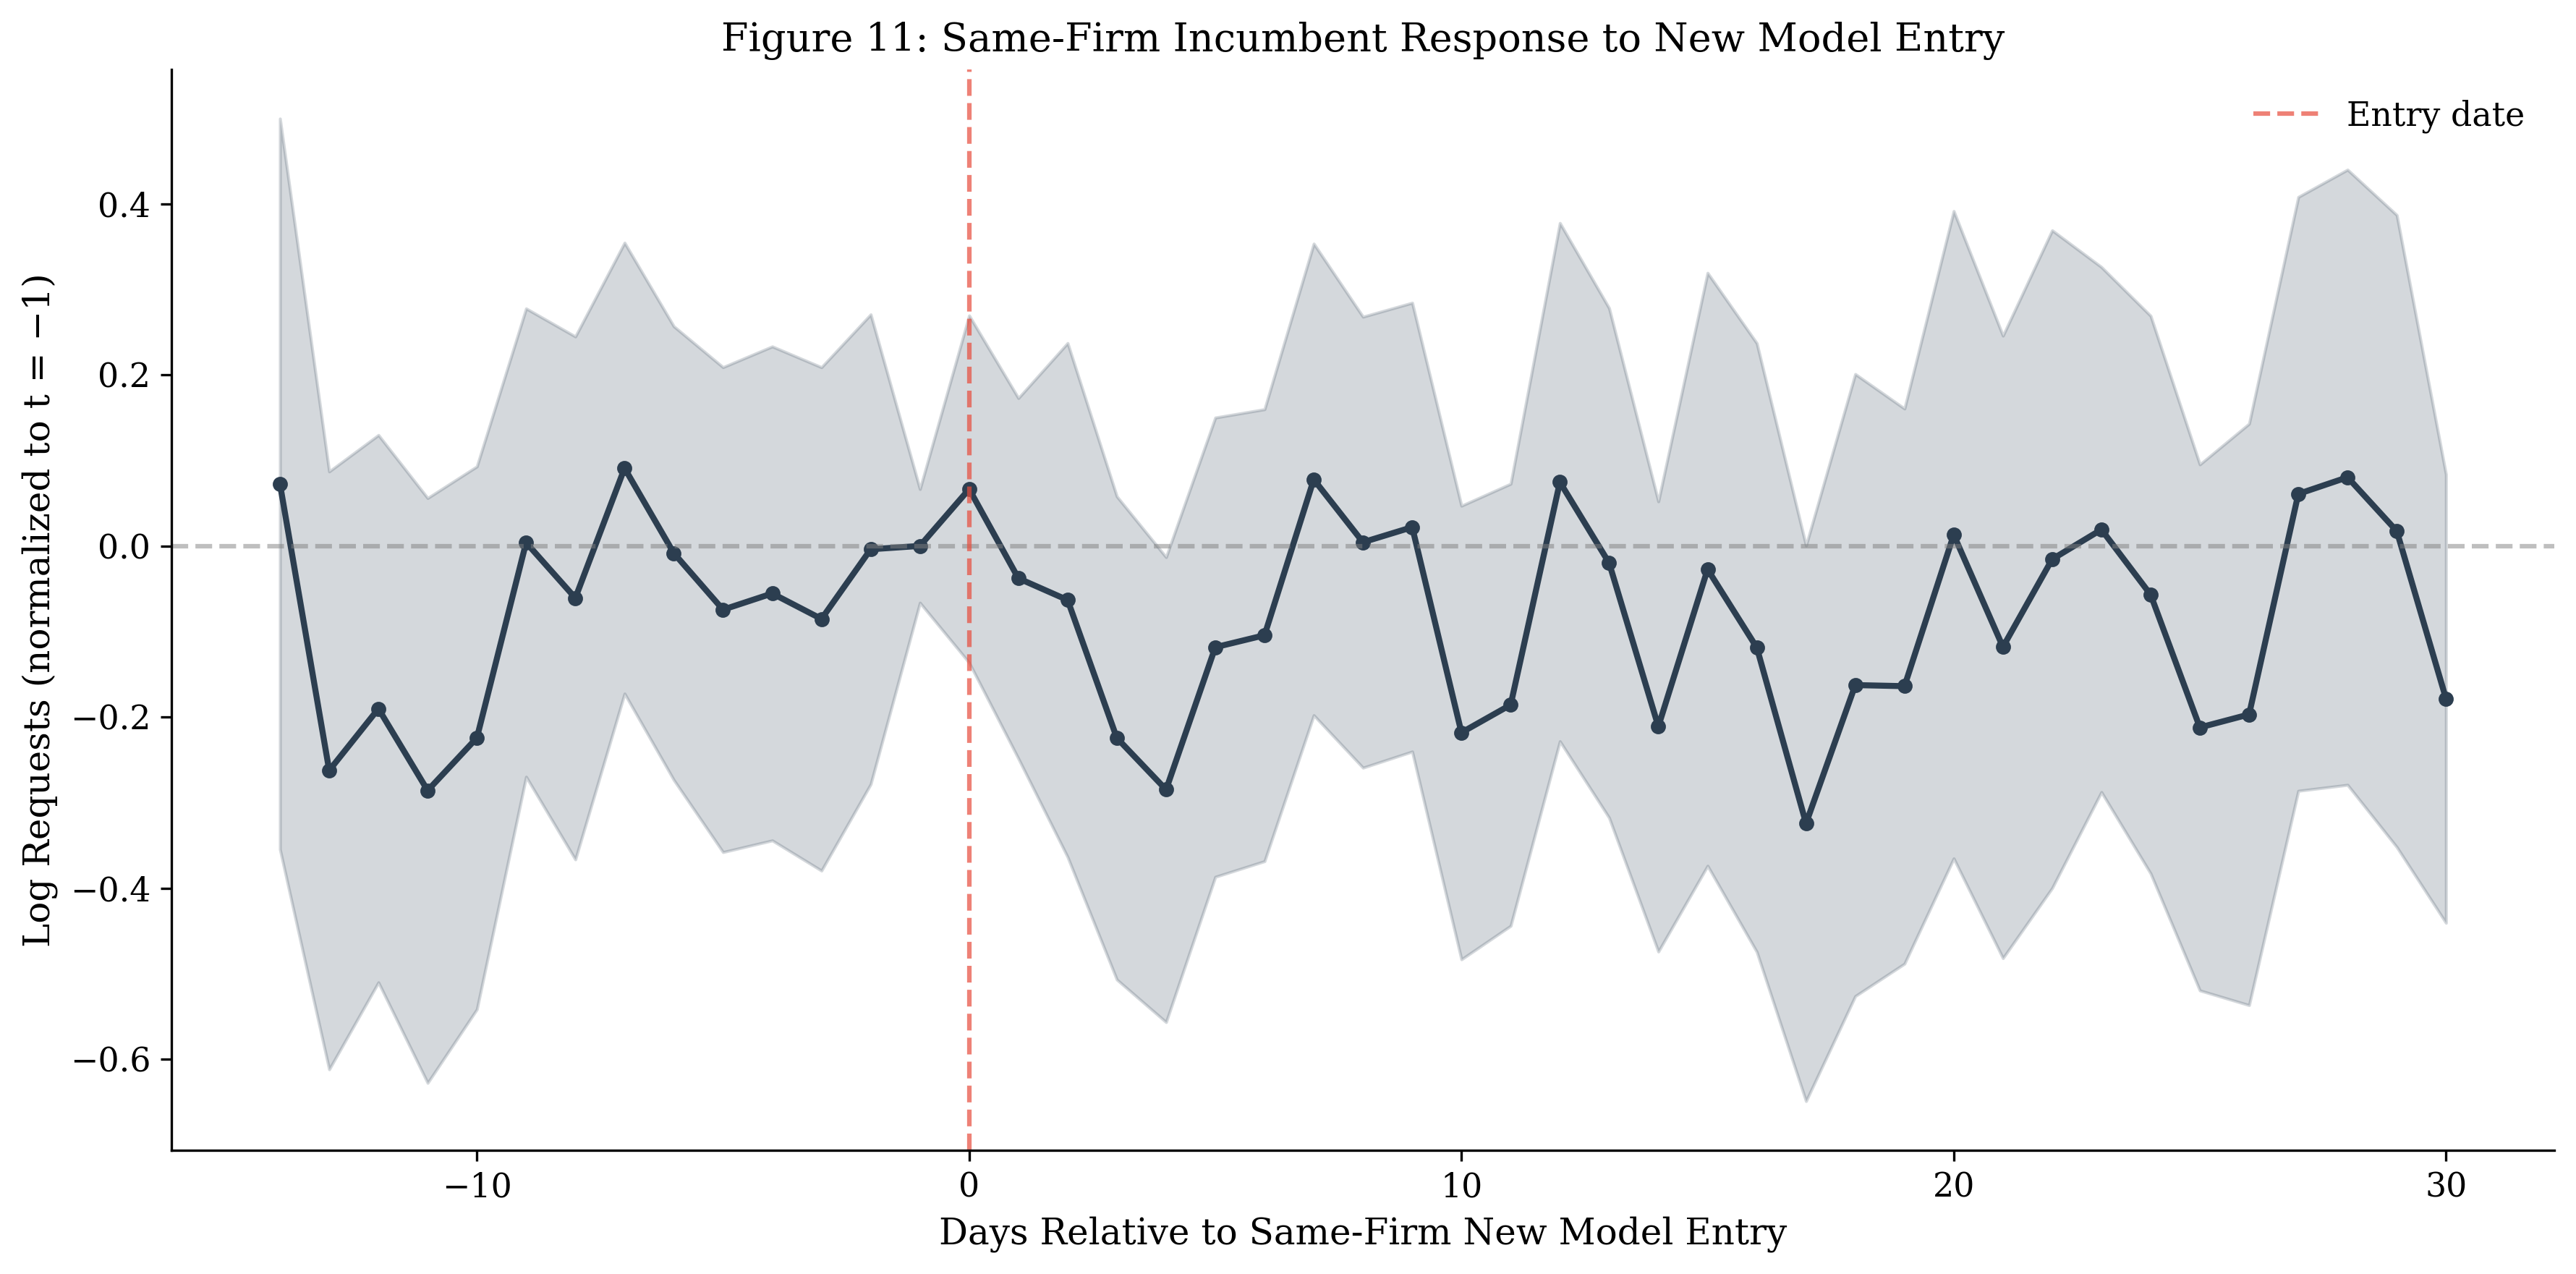
\includegraphics[width=\textwidth]{../output/figures/fig11_event_study_same_firm.png}
\caption{Same-firm entry (all types)}
\label{fig:es_same}
\end{subfigure}
\hfill
\begin{subfigure}[b]{0.48\textwidth}
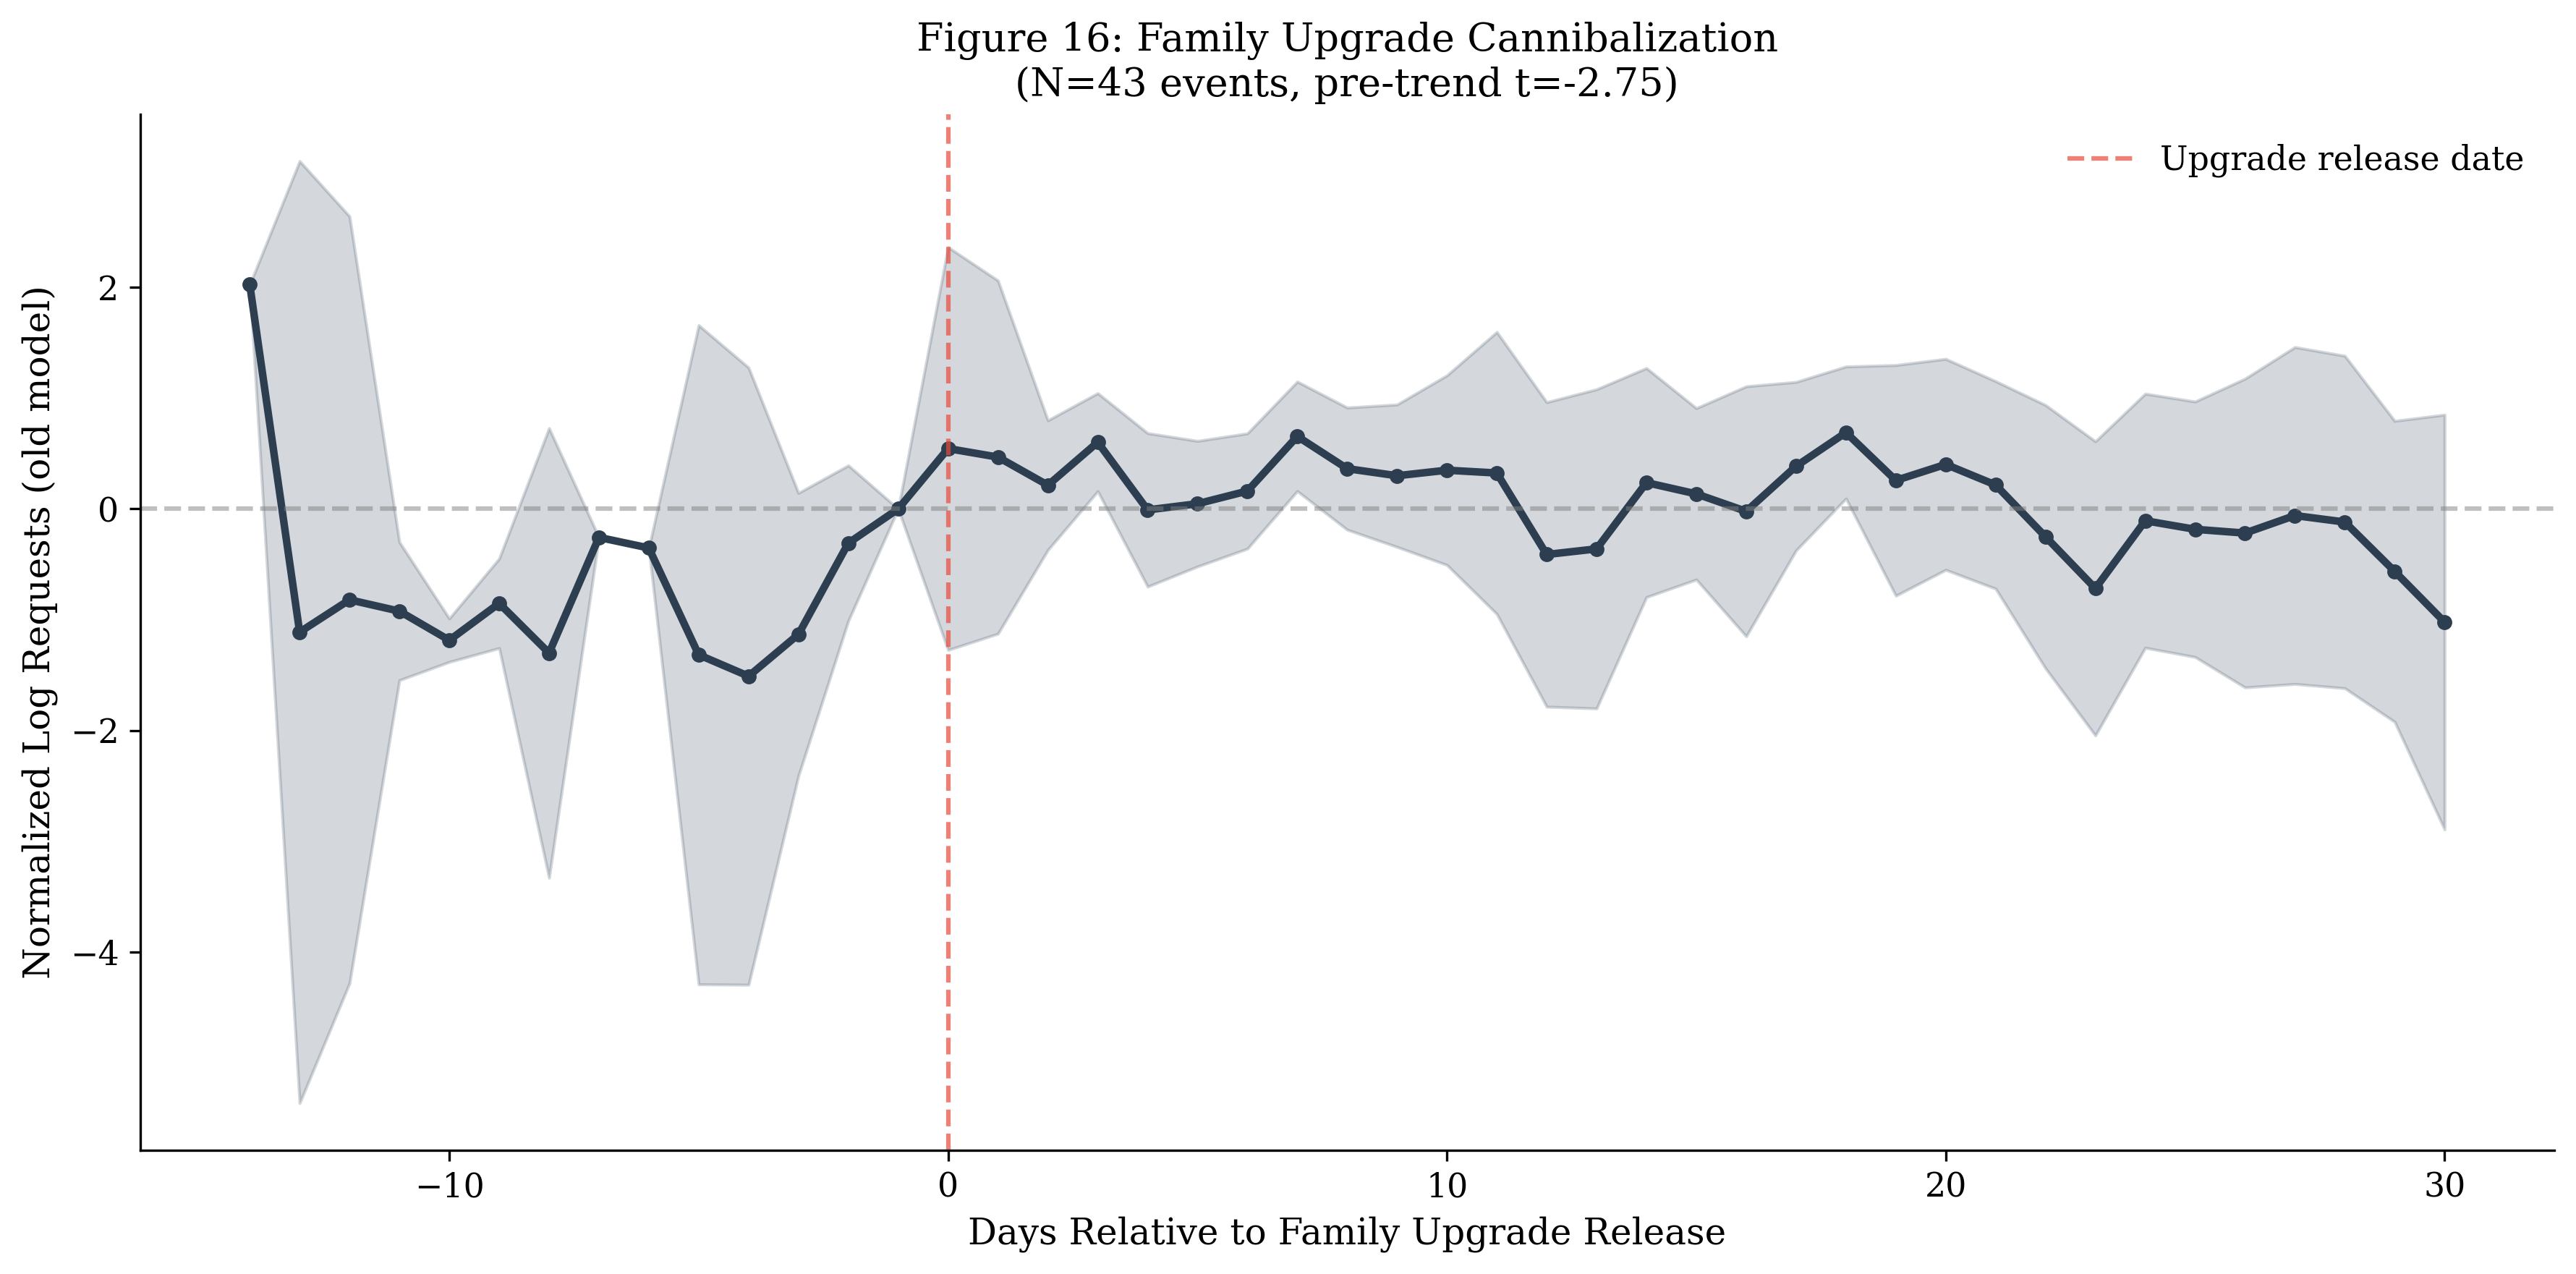
\includegraphics[width=\textwidth]{../output/figures/fig16_family_upgrade_event_study.png}
\caption{Within-family upgrades}
\label{fig:es_family}
\end{subfigure}
\caption{Event Study: Incumbent Model Usage Around Entry Events}
\label{fig:eventstudy}
\vspace{-0.5em}
\par\noindent\small \textit{Notes}: Each point is the estimated coefficient $\hat{\gamma}_k$ from equation~\eqref{eq:eventstudy}, with 95\% confidence intervals. Reference period is $k = -1$ (day before entry). Panel~(a) pools all same-firm entry events ($N_{\text{events}} \approx 98$). Panel~(b) restricts to within-family upgrades. Of the 43 family-upgrade events identified in the panel, only 8 predecessor models have at least 14 pre-event and 30 post-event days of data within our panel, which we require for the event study specification. The small number of events with full event windows produces wide confidence intervals but clear directional patterns.
\end{figure}

The all-entry event study (panel~a) shows no clear pattern: coefficients fluctuate around zero both before and after entry, consistent with the null aggregate result in Table~\ref{tab:entry}. Pre-trend coefficients are noisy but centered near zero, providing no evidence of differential trends before same-firm entry.

The family-upgrade event study (panel~b) tells a different story. Although the small number of upgrade events in the event study figure ($N = 8$ with sufficient pre- and post-event data) produces wide confidence intervals, the \emph{pattern} is informative: predecessor model usage does not trend differentially before the upgrade (days $-14$ to $-1$), then stabilizes or slightly increases in the first week (as the new model ramps up and both coexist), before declining in subsequent weeks as adoption of the successor matures. The dynamic pattern is consistent with a ``coexistence-then-displacement'' narrative: the new model needs time to build adoption, and during this period the predecessor retains its user base. Once the successor is established (typically after 1--2 weeks), users begin migrating, producing the decline captured by our panel regression coefficient. This timing is consistent with the adoption dynamics documented by \citet{fradkin2025demand}, who finds that new model adoption stabilizes within approximately two weeks of release.

The event study also provides a useful check on the timing of displacement. If the estimated decline in predecessor usage appeared \emph{before} the successor's release date, it would suggest that our entry date is mismeasured or that anticipation effects (e.g., users seeing pre-release announcements) are important. We do not observe such pre-event declines in the family-upgrade event study, though the wide confidence intervals mean we cannot rule out modest anticipation effects.

Figure~\ref{fig:es_cross} in the Appendix shows the cross-firm entry event study. Post-entry coefficients are negative on average but noisy and not significantly different from zero at conventional levels.

\subsection{Substitution Across Alternative Nesting Structures}

The firm-based nesting may not be the only---or even the best---way to group models. Table~\ref{tab:altnest} reports nesting parameters under alternative structures.

\begin{table}[H]
\centering
\caption{Nesting Parameter Under Alternative Groupings}
\label{tab:altnest}
\begin{threeparttable}
\begin{tabular}{ldd}
\toprule
Nesting structure & \multicolumn{1}{c}{$\hat{\sigma}$} & \multicolumn{1}{c}{SE} \\
\midrule
By firm (baseline) & 0.456 & (0.042) \\
\quad Reasoning models only & 0.578 & (0.067) \\
\quad Non-reasoning models only & 0.386 & (0.049) \\[4pt]
By capability tier (reasoning vs.\ non-reasoning) & 0.999 & (0.000) \\
By price tier (quartiles) & 0.992 & (0.003) \\
\bottomrule
\end{tabular}
\begin{tablenotes}[flushleft]
\small
\item \textit{Notes}: Each row re-estimates the nested logit with models grouped as indicated. $N = 26{,}444$ for all specifications except the split by capability ($N_{\text{reasoning}} = 10{,}857$; $N_{\text{non-reasoning}} = 15{,}587$). Day fixed effects included. OLS estimates.
\end{tablenotes}
\end{threeparttable}
\end{table}

Two patterns stand out. First, the nesting parameter is substantially higher for reasoning models ($\hat{\sigma} = 0.578$) than non-reasoning models ($\hat{\sigma} = 0.386$). This gap is consistent with more intense within-firm competition in the frontier reasoning segment, where quality differences across providers are smaller and models are more interchangeable.

Second, nesting by capability tier or price tier yields $\hat{\sigma}$ values above 0.99. These boundary estimates should be interpreted with caution. With only two capability-tier nests (reasoning vs.\ non-reasoning) or four price-tier nests, the within-group composition is highly heterogeneous---a reasoning nest contains everything from a small efficient reasoning model to a frontier reasoning system. The within-group share $s_{m|g,t}$ then has enormous cross-sectional variation driven by model heterogeneity \emph{within} groups, which can mechanically push $\hat{\sigma}$ toward the boundary. A multi-level nested logit (e.g., firm nested within capability tier) would better separate these effects, but our sample size limits the precision of such estimates.

That said, the directional result is informative: models sharing the same capability profile or price segment compete more intensely than models in different segments, and this within-segment competition exceeds even within-firm competition ($\hat{\sigma}_{\text{tier}} > \hat{\sigma}_{\text{firm}}$). This is consistent with the intuition that the ``relevant market'' for a reasoning model is the set of all reasoning models, not the set of all models from the same firm. Firm-based nesting captures some of this---since firms tend to specialize within capability--price segments---but understates within-segment substitutability.

\subsection{Robustness}

Table~\ref{tab:robustness} summarizes robustness checks on the nested logit and panel regression results.

\begin{table}[H]
\centering
\caption{Robustness Checks}
\label{tab:robustness}
\begin{threeparttable}
\begin{tabular}{lddl}
\toprule
Check & \multicolumn{1}{c}{Estimate} & \multicolumn{1}{c}{SE} & $N$ \\
\midrule
\multicolumn{4}{l}{\textit{Panel A: Panel regression---same-firm entry $[0,7]$}} \\
(1) DV: Log tokens & 0.001 & (0.003) & 30,699 \\
(2) DV: Log market share & -0.001 & (0.003) & 30,903 \\
(3) High-volume models only & 0.002 & (0.006) & 13,762 \\
(4) 7-day rolling avg DV & -0.001 & (0.003) & 30,133 \\
(5) Exclude first/last 7 days & -0.001 & (0.005) & 26,164 \\
(6) Placebo: shuffled firm labels & 0.002 & (0.003) & 30,903 \\[4pt]
\multicolumn{4}{l}{\textit{Panel B: Nested logit sensitivity}} \\
(7) Outside option 10\% & 0.456 & (0.042) & 26,444 \\
(8) Outside option 40\% & 0.456 & (0.042) & 26,444 \\
(9) Oster $\delta$ & \multicolumn{2}{c}{154.9} & \\
\bottomrule
\end{tabular}
\begin{tablenotes}[flushleft]
\small
\item \textit{Notes}: Panel A reports the same-firm entry $[0,7]$ coefficient under alternative specifications. Panel B reports the nesting parameter under alternative outside option assumptions and the Oster (2019) stability bound. Baseline nested logit: $\hat{\sigma} = 0.456$ (SE $= 0.042$).
\end{tablenotes}
\end{threeparttable}
\end{table}

The panel regression null is robust across all checks: replacing the dependent variable with log tokens, log market share, or a 7-day rolling average; restricting to high-volume models; trimming panel edges; and running a placebo test with shuffled firm labels (which correctly produces a near-zero coefficient). The nested logit nesting parameter is invariant to the outside option share assumption---$\hat{\sigma} = 0.456$ whether we set the outside option at 10\%, 20\%, or 40\% of total market size. The Oster $\delta = 155$ reinforces the stability of the OLS estimate.

A leave-one-firm-out analysis (Appendix Table~\ref{tab:lofo}) shows that the same-firm entry coefficient does not change materially when any single major firm (Google, OpenAI, Mistral, Minimax, or DeepSeek) is excluded, confirming that the null is not driven by one firm's idiosyncratic entry pattern. The largest deviation occurs when excluding OpenAI ($\hat{\beta} = -0.005$, SE $= 0.005$), which is still economically small and statistically insignificant.

The placebo test deserves additional comment. We randomly shuffled firm labels across models while preserving the panel structure, then re-estimated the same-firm entry coefficient. The resulting estimate ($\hat{\beta} = 0.002$, SE $= 0.003$) is indistinguishable from zero, confirming that the null result in our main specification is not a mechanical artifact of the panel structure or the entry variable construction. If the same-firm entry variable were picking up market-wide trends that happen to coincide with entry events, the placebo would also show a non-zero coefficient; it does not.

We also considered potential bias from staggered treatment timing \citep{dechaisemartin2020twoway, goodmanbacon2021}. In our setting, the concern is that early entrants' displacement effects may differ from late entrants' effects, and TWFE could produce a weighted average that misrepresents both. The event-by-event heterogeneity in our event study plots (Figures~\ref{fig:eventstudy} and~\ref{fig:es_cross}) shows substantial variation across events, consistent with heterogeneous treatment effects. However, because our aggregate coefficient is approximately zero, the TWFE weighting issue is less consequential than in settings where the coefficient is significantly different from zero: a weighted average of effects near zero remains near zero regardless of the weights.

\subsection{Market Expansion}

Although our primary focus is on the reallocation of \emph{existing} demand, we briefly document patterns in market expansion. Using weekly data from the rankings snapshots, total platform requests grew approximately 20\% over our 93-day sample period. In weeks containing a major model launch (defined as a model reaching the top 50 within 7 days of entry), total platform requests were 3--20\% higher than the weekly trend, though the confidence intervals are wide and the number of such events is small.

This is consistent with H3 and with \citet{fradkin2025demand}, who documents that some model releases expand the market (Gemini 2.5 Pro) while others primarily reshuffle existing demand (Gemini 2.0 Flash). Our panel is too short and our identification too weak to distinguish demand-expanding entries from mere coincidence with growth trends, so we flag this as suggestive evidence rather than a firm conclusion.

% === 7. DISCUSSION ===
\section{Discussion}
\label{sec:discussion}

\subsection{Economic Interpretation}

The central finding of this paper is that creative destruction in the LLM API market operates almost exclusively through \emph{within-family upgrades}. When a firm releases a new generation in an existing model family, the predecessor is associated with roughly one-third fewer requests. All other forms of entry---new product lines from the same firm, models from rival firms---produce no measurable displacement in the short run.

This pattern has a natural interpretation through the lens of vertical differentiation \citep{shaked1982relaxing}. Within a model family, successive generations represent movement along a single quality ladder: Claude 3.5 Sonnet improves on Claude 3 Sonnet along most dimensions (speed, accuracy, context window). Users who adopted the earlier version have revealed a preference for models in that capability range at that price point; the upgrade directly addresses their use case. The decision to switch is straightforward---same API format, same pricing structure, better performance.

Cross-firm and cross-family entries, by contrast, represent entry on a \emph{different} quality ladder. A user of Claude 3 Sonnet may find GPT-4o attractive in principle, but the switching cost---even on OpenRouter, where it is minimal in technical terms---involves evaluating a different model's strengths, adjusting prompt strategies, and potentially changing downstream processing. These frictions, small as they are, appear sufficient to prevent measurable short-run displacement.

The nesting parameter $\hat{\sigma} = 0.46$ provides a structural confirmation. Within-firm models are nearly twice as substitutable as cross-firm models, but far from perfect substitutes ($\sigma \ll 1$). The firm nesting structure captures real demand-side grouping: users cluster by provider ecosystem. But the near-unity nesting parameters under capability-tier and price-tier groupings ($\hat{\sigma} > 0.99$) reveal that the deeper competitive margin is defined by what models \emph{do} and what they \emph{cost}, not who makes them. Firms happen to specialize within capability--price segments, so firm-based nesting is a reasonable approximation, but it understates within-segment substitutability.

\subsection{Comparison with Existing Findings}

Our results are broadly consistent with \citet{fradkin2025demand}, who documents heterogeneous substitution patterns across three model releases. His finding that Claude 3.7 Sonnet ``primarily stole share from Claude 3.5 Sonnet'' (intra-family cannibalization) aligns with our systematic estimate of the family-upgrade channel. His finding that Gemini 2.5 Pro expanded the market while Gemini 2.0 Flash primarily reshuffled demand aligns with our suggestive evidence on capability-driven expansion. Our contribution is to show that these patterns are not idiosyncratic to specific releases but reflect a systematic structural feature of demand substitution in this market.

The price elasticity implied by our nested logit ($\hat{\alpha} = 0.26$ on the log-share equation) is somewhat lower than the unit elasticity reported by \citet{demirer2025emerging}, though the specifications differ enough to make direct comparison imprecise. Their estimate uses market-level variation over a longer horizon and includes both OpenRouter and Azure data; ours conditions on model characteristics and uses daily cross-sectional variation on OpenRouter alone.

Our findings complement the historical technology-market literature. \citet{bresnahan1999technological} documents that platform displacement in computing (mainframes to PCs) took decades. The LLM market compresses this timeline dramatically: within-family displacement is largely complete within two weeks of a successor's release. The market's low switching costs and rapid iteration cycles produce a form of Schumpeterian dynamics that is qualitatively similar to---but quantitatively far faster than---historical precedents.

\subsection{Relationship to Theory}

Our findings map onto the theoretical framework in Section~\ref{sec:theory} as follows. H1 (cannibalization dominance) receives partial support: the nesting parameter $\sigma = 0.46$ confirms that within-firm models are closer substitutes, and the family-upgrade coefficient shows that cannibalization is large \emph{when it occurs}. But the aggregate same-firm entry effect is null because most same-firm entries are different-family entries that do not compete with existing models. The ``cannibalization dominance'' prediction holds for within-family upgrades but not for the broader category of same-firm entry.

H2 (quality-ladder concentration) receives strong support. The family-upgrade coefficient of $-0.43$ compared to the different-family coefficient of zero is exactly what vertical differentiation theory predicts: consumers trade up along a quality ladder, and models on different ladders coexist. The near-unity nesting parameters under capability-tier and price-tier groupings reinforce this: the ``true'' competitive segments in this market are defined by capability and price, not firm identity.

H3 (capability-driven expansion) receives suggestive but imprecise support. We observe positive market-level growth around major launches, but cannot cleanly separate expansion from secular trend growth with our identification strategy.

The pattern of creative destruction we document---vertical displacement within product families, horizontal coexistence across families---resembles the ``quality ladder'' dynamics modeled by \citet{baron2020vertical} and the ``Schumpeterian competition'' described by \citet{bresnahan2011schumpeterian} in the context of IBM and Microsoft. The distinctive feature of the LLM market is the \emph{speed} of these dynamics: what took years in the PC industry takes days in the LLM API market.

\subsection{Policy Implications}

We offer three observations, framed with appropriate caution given the descriptive nature of our evidence.

First, the concentration of displacement within model families suggests that \emph{self-competition} is the primary discipline on market power in the current LLM market. Firms face competitive pressure primarily from their own next-generation models, not from rivals. This is consistent with \citet{arrow1962economic}'s replacement effect and may partly explain the rapid pace of model releases: firms must keep upgrading to retain their user base.

Second, the near-zero cross-firm displacement effect---even in a setting with minimal switching costs---suggests that the market is either still in a rapid growth phase (where entry is accommodated by expansion rather than displacement) or that horizontal differentiation across providers is sufficient to insulate firms from each other's entries. Either interpretation implies that the market is currently far from the ``winner-take-all'' dynamic that some observers have predicted.

Third, the near-perfect within-tier substitution ($\hat{\sigma} > 0.99$) implies that models competing on the same capability--price frontier face intense competition, even if their providers are different firms. This has implications for pricing: firms with models in crowded tiers face more elastic demand than firms occupying unique capability--price positions.

\subsection{Limitations}

We note five specific limitations that bound the conclusions of this analysis.

\paragraph{Short panel.} Our data span 93 days. If cross-firm displacement operates on longer timescales---as in traditional technology markets \citep{bresnahan1999technological}---our event windows may be too short to detect it. The family-upgrade event study shows some decline persisting through day 30, but our panel provides no window into month-to-month or quarter-to-quarter dynamics.

\paragraph{Platform selection.} OpenRouter users are developers who value multi-model access and low switching costs. Enterprise customers with direct API contracts face higher switching costs and may exhibit different substitution patterns. Our estimates are an upper bound on displacement effects in the broader market.

\paragraph{No causal identification.} The entry timing of new models is not exogenous. Our panel regressions are best interpreted as conditional correlations, and the nested logit estimates rely on cross-sectional variation in shares and characteristics rather than experimental price or quality variation. The failure of our BLP-style instrument underscores the difficulty of finding credible exclusion restrictions in this setting.

\paragraph{Small number of family-upgrade events.} The family-upgrade coefficient ($\hat{\beta} = -0.43$, $N_{\text{events}} = 43$) is precisely estimated but based on a modest number of events. Future data with more upgrade cycles would permit more granular analysis of heterogeneity across model families.

\paragraph{No supply-side model.} We do not model firms' decisions about when and what to release. The strategic timing of model releases---which our analysis takes as given---is itself an important economic object. A richer framework that endogenizes entry would allow welfare analysis and counterfactual simulations, but requires data on development costs and firm objectives that we lack. The absence of a supply-side model also means we cannot assess the welfare implications of the cannibalization pattern: whether the observed pace of model upgrades is socially efficient---or whether firms over-invest in incremental upgrades at the expense of more fundamental innovations---is an open question that our data cannot address.

\paragraph{Model deprecation.} An important caveat is that some predecessor models may be deprecated or removed by their providers after an upgrade, in which case the measured ``displacement'' conflates demand reallocation with supply-side removal. On OpenRouter, deprecated models generally remain available as long as the underlying provider continues serving them, but providers occasionally discontinue older model versions. We cannot distinguish demand-driven migration from forced migration due to deprecation in our data. To the extent that some of the family-upgrade displacement reflects supply-side removal rather than demand-side choice, our estimates overstate the degree to which users voluntarily abandon predecessor models.

\paragraph{Measurement limitations.} Our usage data measure request counts and token volumes at the model level, but we lack information on the \emph{quality} of interactions (e.g., user satisfaction, task completion rates) and on the downstream value generated by different models. A model that receives fewer requests but serves higher-value tasks may generate more economic surplus than a high-traffic model used for simple completions. Our analysis of demand reallocation is therefore a quantity-based measure that does not capture value-weighted substitution patterns. Additionally, we observe usage through a single platform; the same developer may use different models through different channels (direct API, other aggregators), and our platform-specific data cannot capture this multi-platform usage.

% === 8. CONCLUSION ===
\section{Conclusion}
\label{sec:conclusion}

This paper documents how demand reallocates when new LLMs enter the API marketplace. Using daily data on 385 models from 66 firms over 93 days on OpenRouter, we estimate a nested logit demand model and conduct descriptive panel regressions around entry events.

The core finding is that creative destruction in this market is \emph{vertical and intra-firm}: each model generation replaces the last within its product family, while models on different quality ladders---whether from the same firm or from rivals---coexist with little mutual displacement. The nesting parameter of 0.46 confirms moderate within-firm substitution, but the near-unity parameters under capability-tier and price-tier groupings reveal that the deeper competitive margin is defined by what a model can do and what it costs.

Taken together, our demand estimates and entry-event analysis paint a consistent picture of how this market functions at the micro level. These results describe a market in early-stage rapid growth, where entry is accommodated primarily by market expansion rather than displacement. Whether cross-firm displacement emerges as the market matures---as it did in the PC revolution documented by \citet{bresnahan1999technological}---remains an open question that longitudinal data will eventually answer. For now, the LLM API market appears to be one where firms compete primarily with themselves, upgrading along quality ladders in a rapid succession of model generations, while the broader competitive landscape remains remarkably stable on a day-to-day basis.

Three directions for future research stand out. First, longer panels would permit analysis of medium- and long-run displacement dynamics that our 93-day window cannot capture. As the LLM market matures and growth rates decline, cross-firm displacement may become more prominent---as it did in the PC industry during the transition from rapid growth to steady state \citep{bresnahan1999technological}. A panel spanning multiple years would allow researchers to test whether the ``cannibalization dominance'' result reflects a structural feature of the market or merely the current growth phase.

Second, combining demand-side analysis with supply-side data on development costs and release timing would enable structural models of entry and innovation incentives. The strategic timing of model releases is itself an economically interesting object: do firms accelerate releases in response to rival entry, or do they follow an internal development cadence that is largely independent of market conditions? Our data cannot answer this question because we observe only the release dates, not the decision process behind them. But the observation that rival entry produces no short-run displacement suggests that defensive release timing---rushing a model to market to preempt a competitor---may be less important in this market than in others.

Third, data from direct API providers (not just aggregators) would allow researchers to study displacement across the full spectrum of switching costs, from the near-zero costs on OpenRouter to the substantial frictions facing enterprise customers with deeply integrated deployments. If displacement effects are substantially smaller for direct-API customers, this would confirm that the near-zero switching costs on OpenRouter are a first-order feature of our results and not merely an incidental platform characteristic.

Finally, the LLM market's rapid evolution creates a rare opportunity for quasi-experimental identification. Exogenous capability jumps---such as the sudden availability of reasoning capabilities in late 2024, or unexpected breakthrough models from new entrants---could provide instruments for future work. As the literature on LLM market economics develops, the combination of high-frequency data, frequent entry events, and rapid capability advancement makes this setting unusually rich for empirical industrial organization research. The LLM API market is, in effect, a laboratory for studying Schumpeterian competition in real time---one where the traditional barriers to high-frequency analysis of product entry and displacement (long product cycles, infrequent entry, sparse data) are absent. Our paper takes a first step toward systematic analysis of this laboratory; much remains to be learned.

\singlespacing
\bibliography{references}

% === APPENDIX ===
\newpage
\begin{appendices}
\section{Additional Figures}

\begin{figure}[H]
\centering
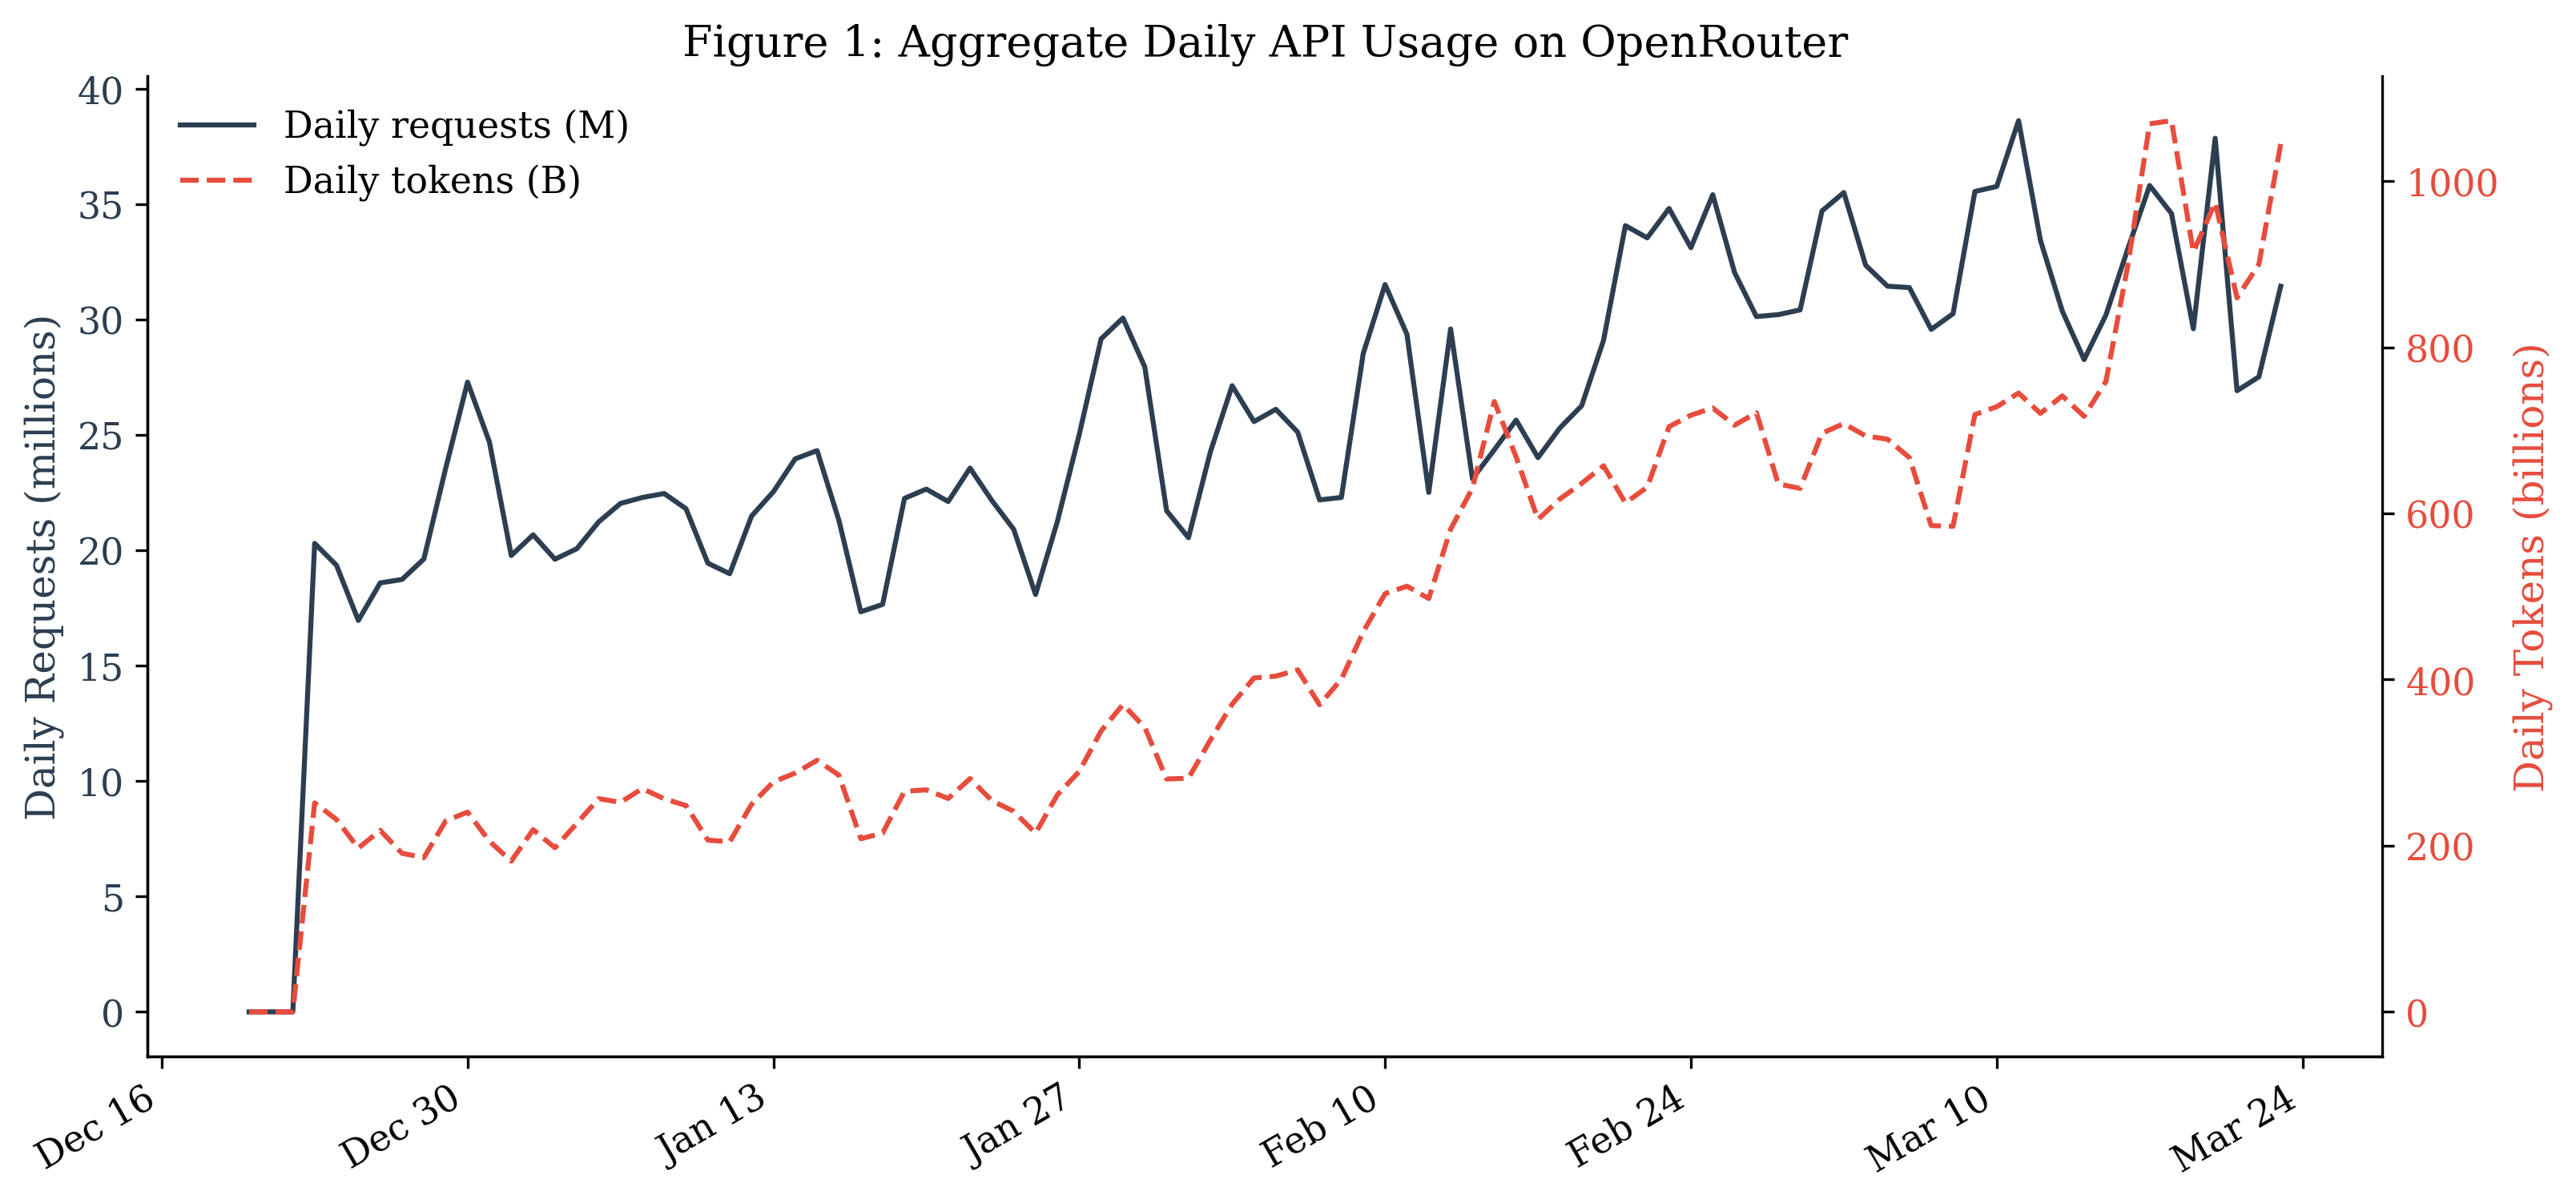
\includegraphics[width=0.85\textwidth]{../output/figures/fig01_aggregate_trends.png}
\caption{Aggregate Daily Requests and Tokens Over Time}
\label{fig:aggregate}
\par\noindent\small \textit{Notes}: Daily total requests and total tokens processed on OpenRouter, December 2025 to March 2026. Both series show strong upward trends with weekday--weekend cyclicality.
\end{figure}

\begin{figure}[H]
\centering
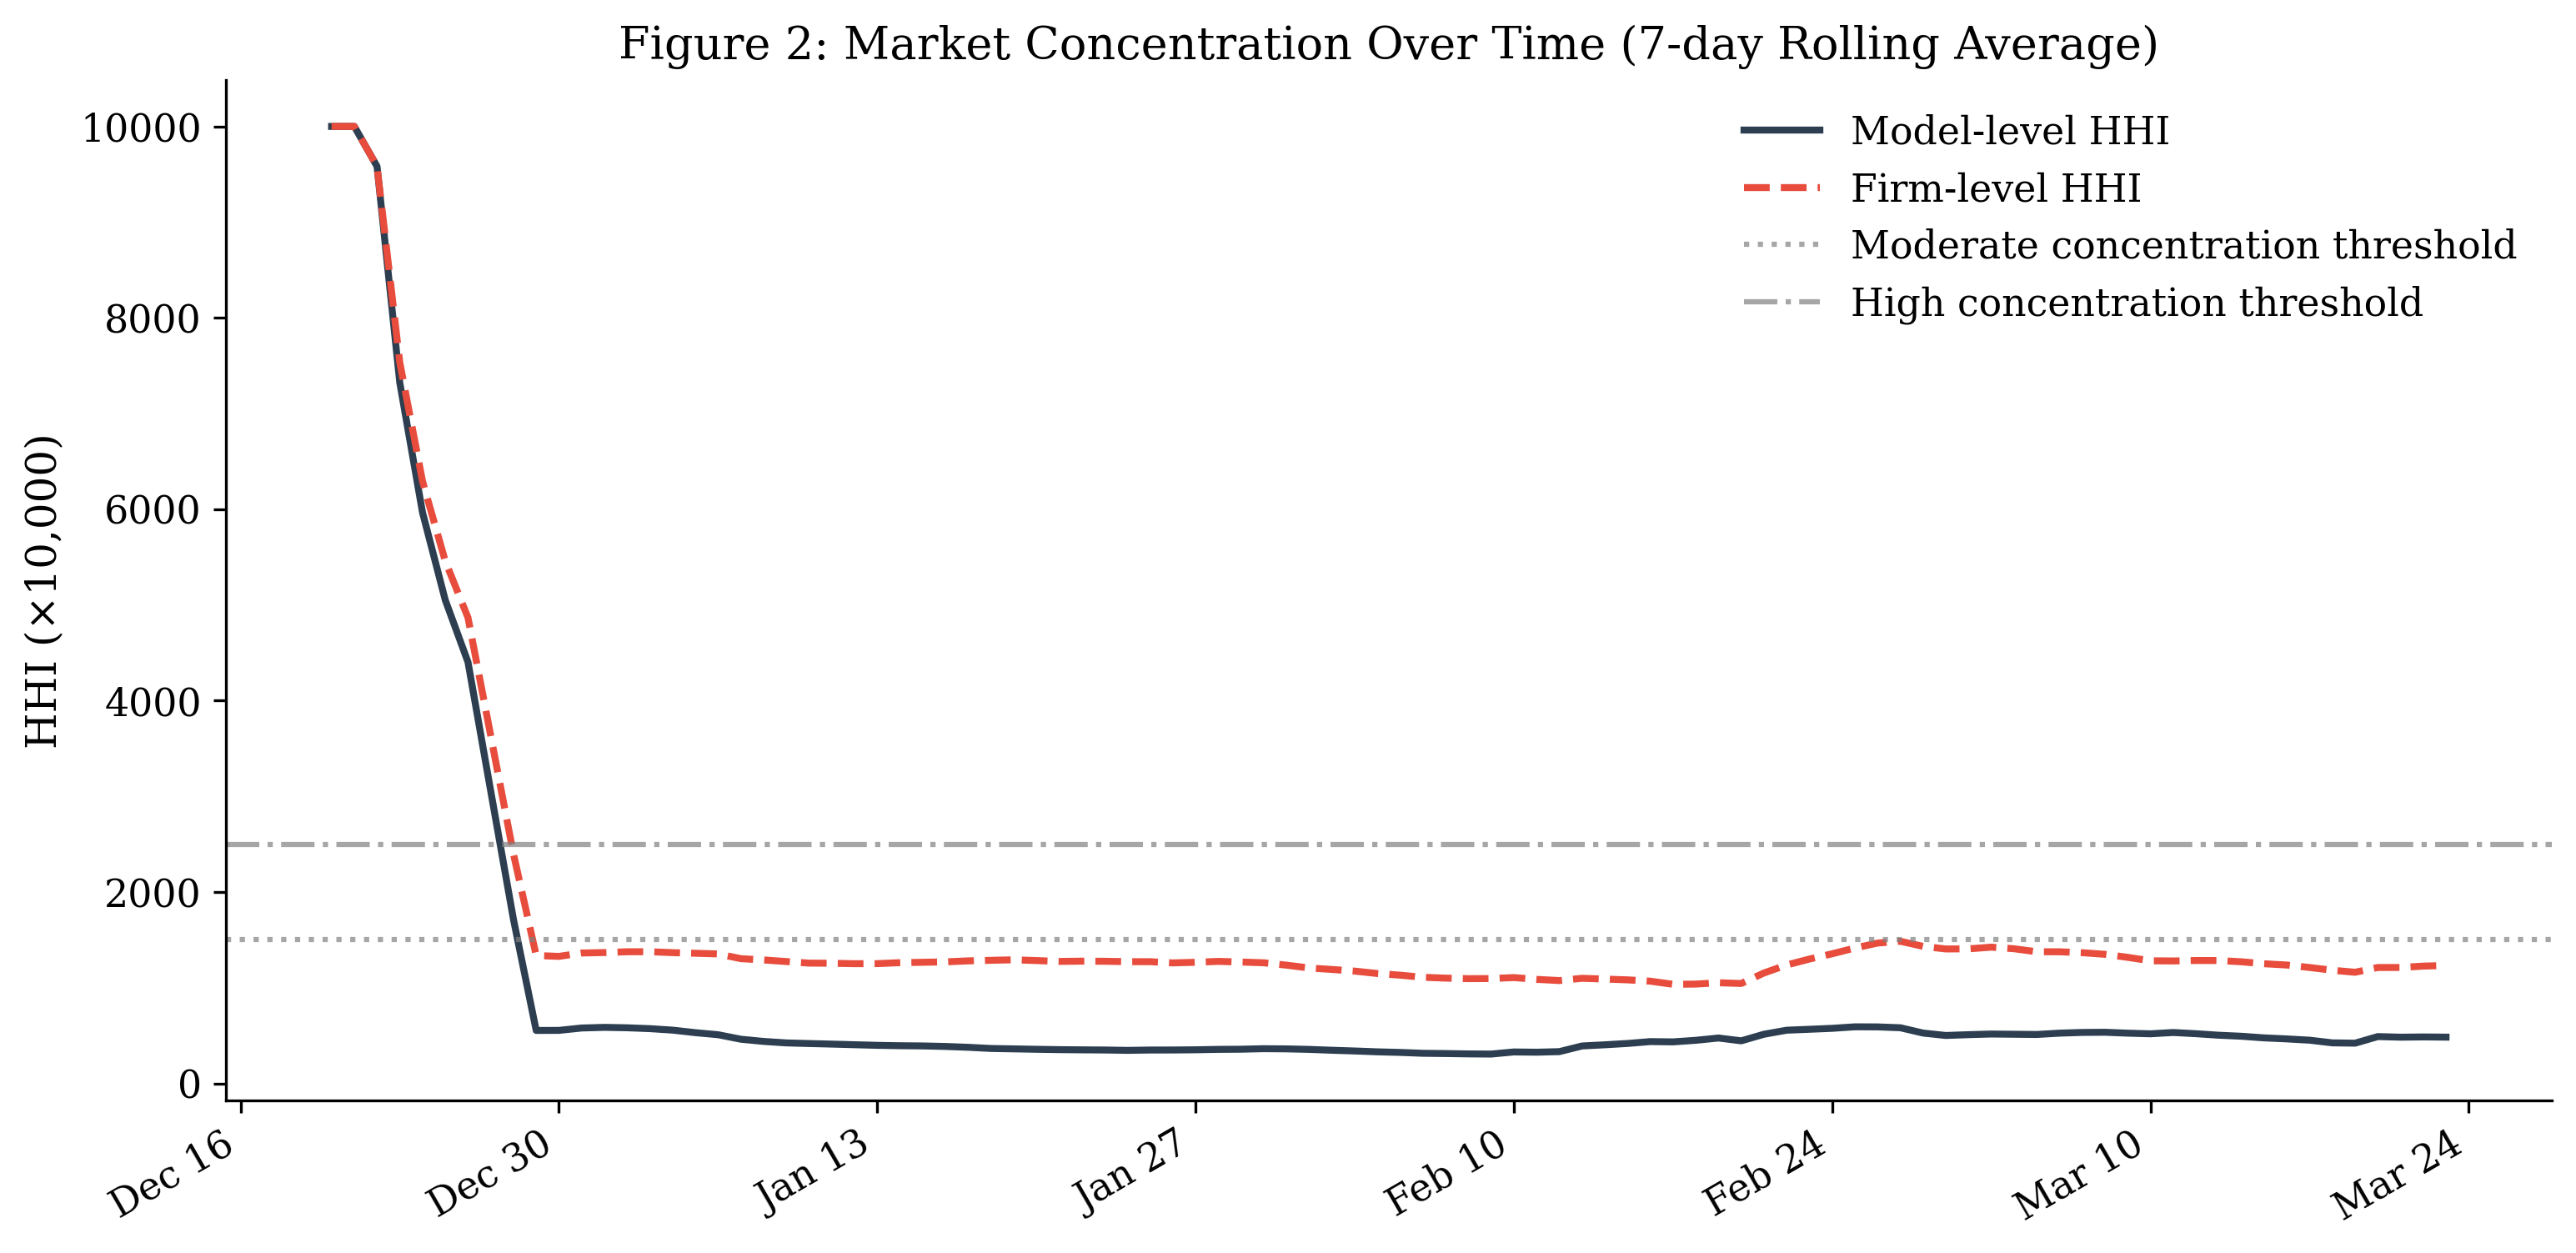
\includegraphics[width=0.85\textwidth]{../output/figures/fig02_hhi_over_time.png}
\caption{Market Concentration Over Time (HHI)}
\label{fig:hhi}
\par\noindent\small \textit{Notes}: Herfindahl-Hirschman Index computed at the model level and firm level, using daily request shares. The model-level HHI averages 741 and the firm-level HHI averages 1,524.
\end{figure}

\begin{figure}[H]
\centering
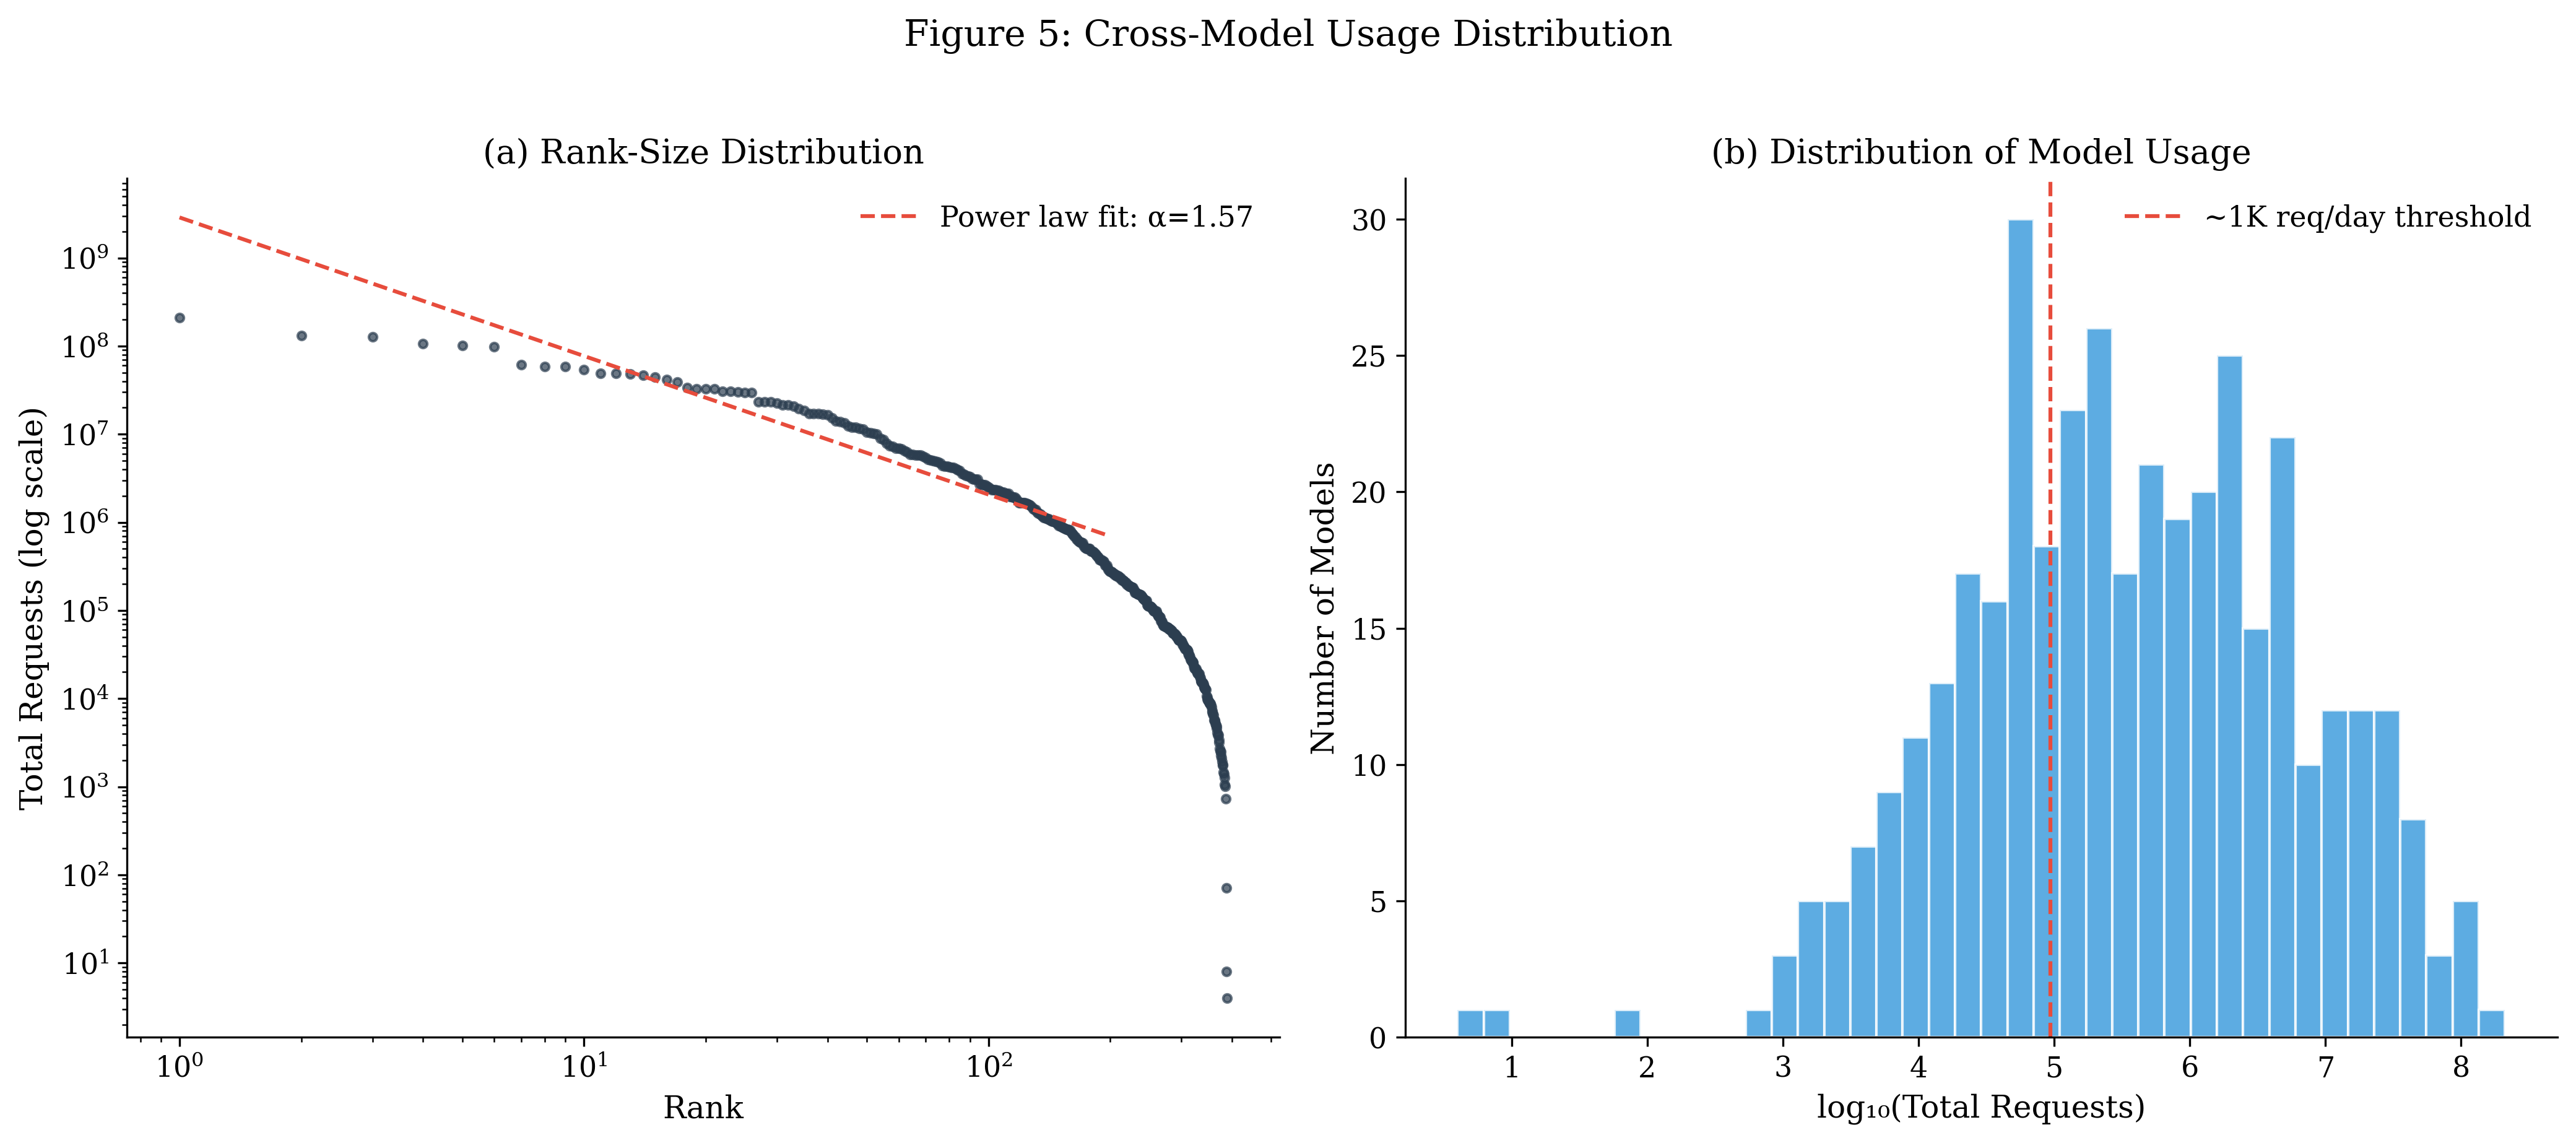
\includegraphics[width=0.85\textwidth]{../output/figures/fig05_usage_distribution.png}
\caption{Rank-Size Distribution of Model Usage}
\label{fig:ranksize}
\par\noindent\small \textit{Notes}: Log-log plot of model rank (by total requests) against total requests over the sample period. The fitted power-law exponent is $\alpha = 1.57$.
\end{figure}

\begin{figure}[H]
\centering
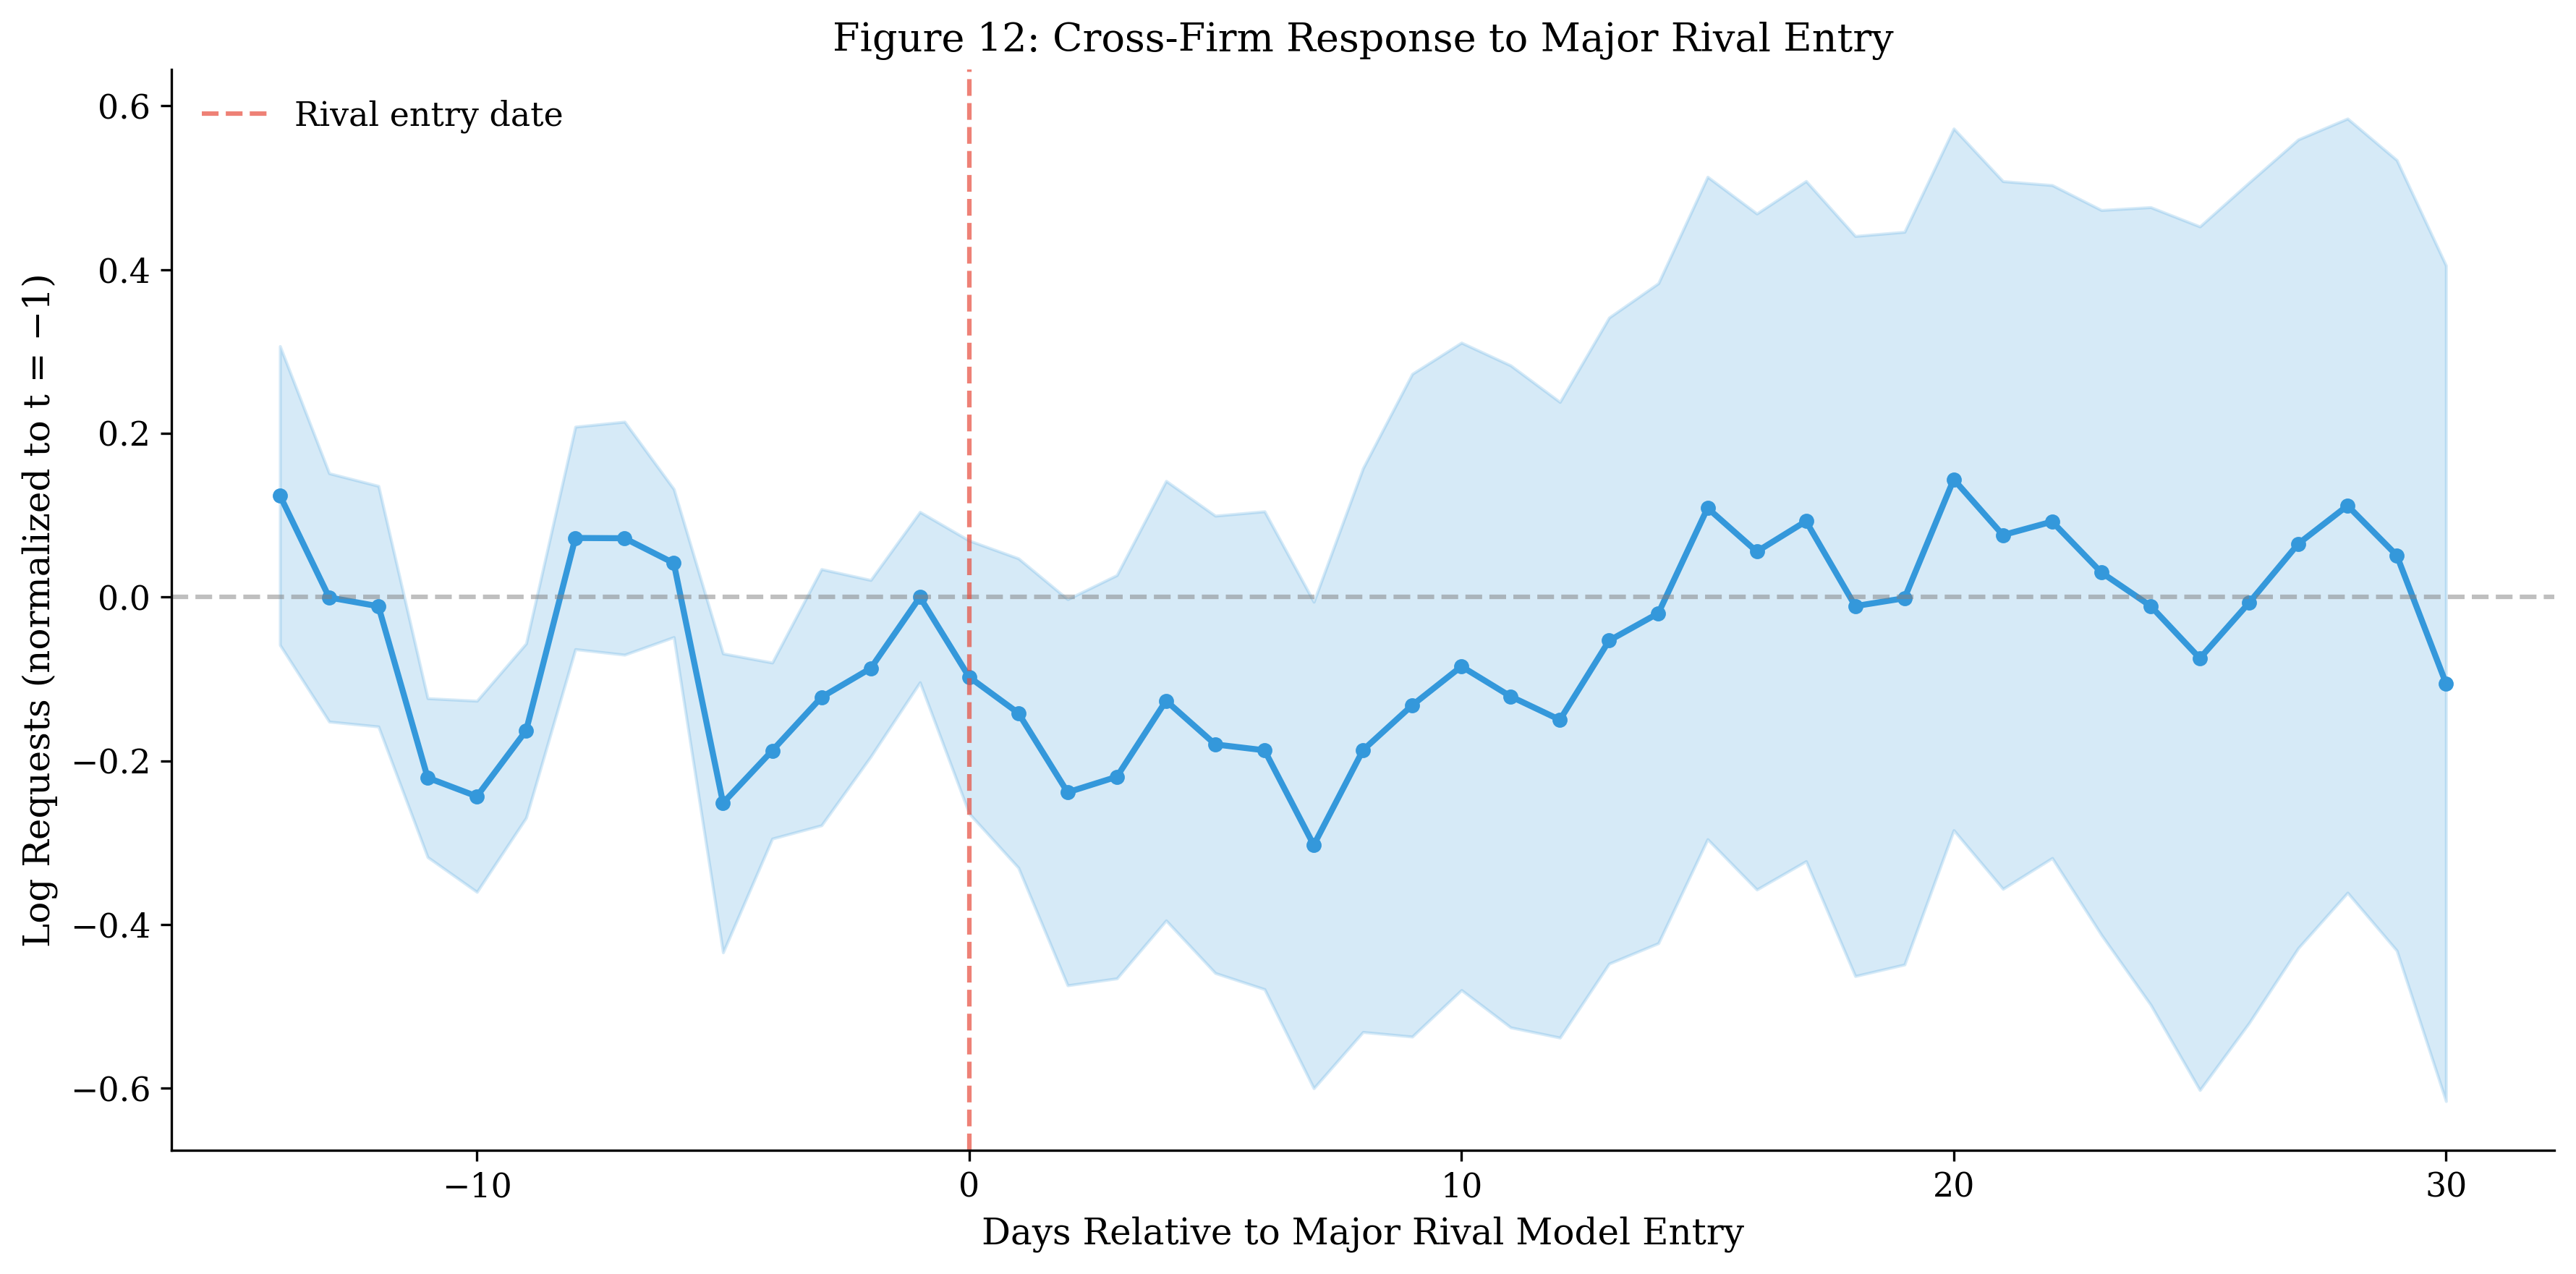
\includegraphics[width=0.85\textwidth]{../output/figures/fig12_event_study_cross_firm.png}
\caption{Event Study: Cross-Firm Entry}
\label{fig:es_cross}
\par\noindent\small \textit{Notes}: Event study coefficients for incumbent model usage around cross-firm entry events. Reference period is $k = -1$. Post-entry coefficients are negative on average but noisy and not significantly different from zero.
\end{figure}

\begin{figure}[H]
\centering
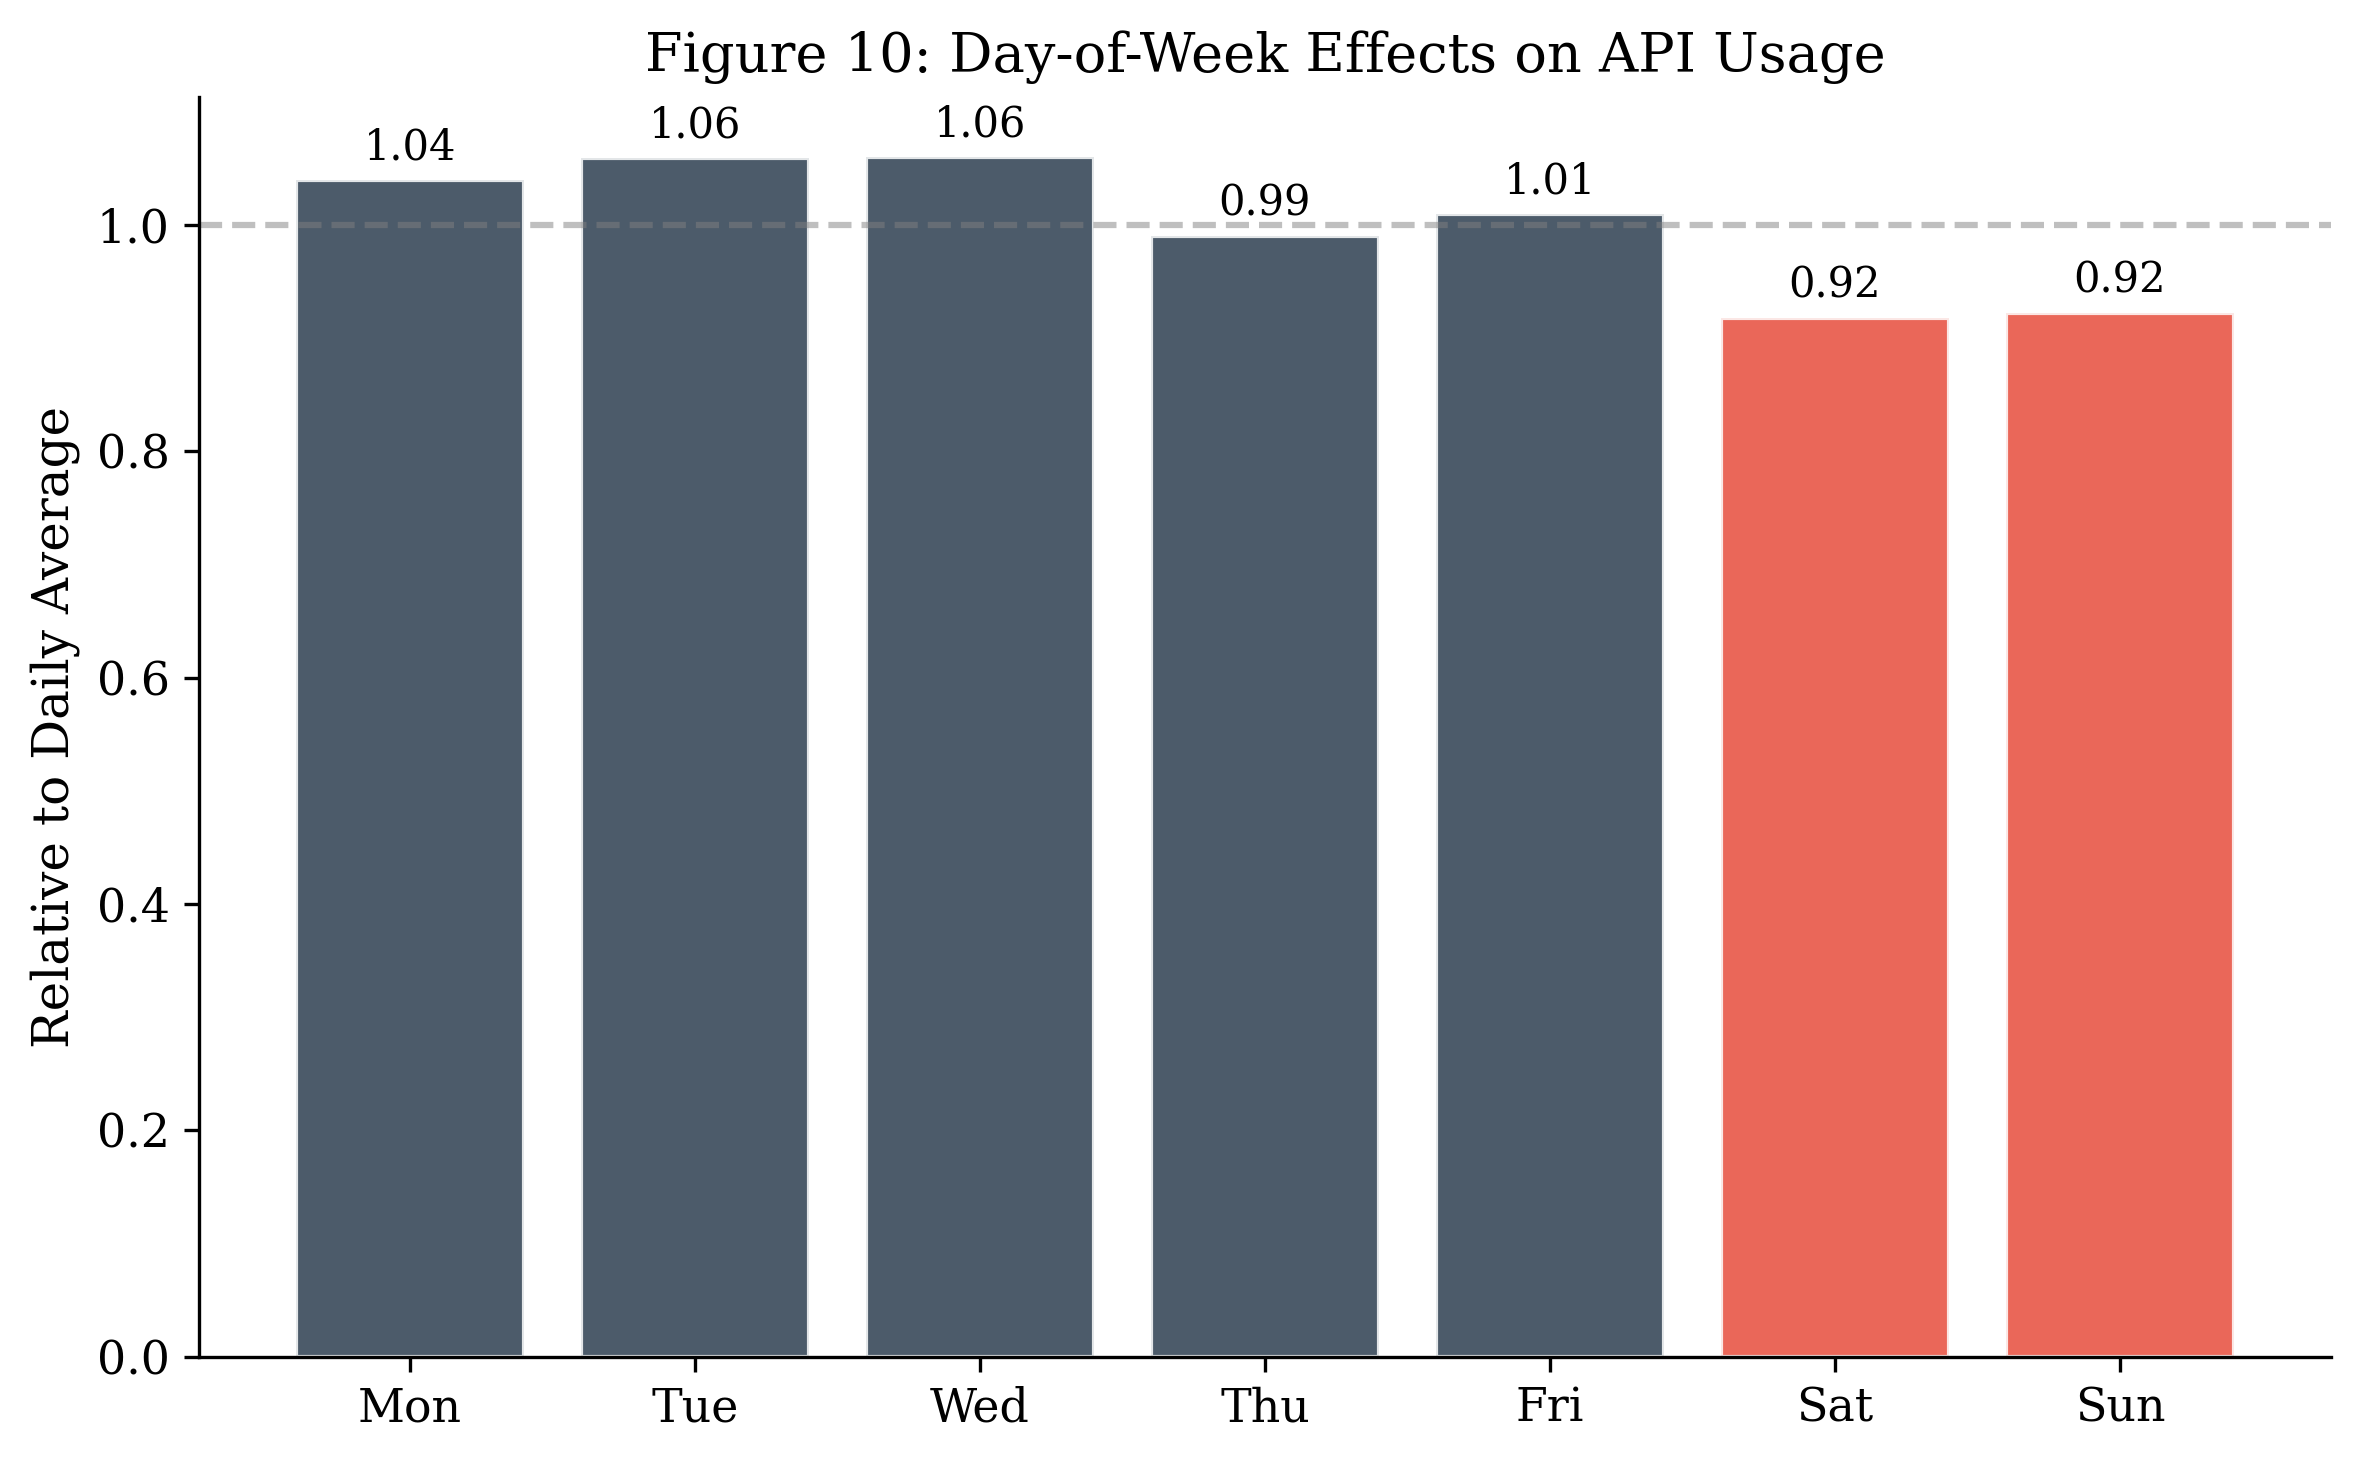
\includegraphics[width=0.85\textwidth]{../output/figures/fig10_weekday_effects.png}
\caption{Day-of-Week Usage Patterns}
\label{fig:weekday}
\par\noindent\small \textit{Notes}: Average daily requests by day of week, normalized to the overall daily mean. Weekdays run 3\% above average; weekends run 8\% below.
\end{figure}

\begin{figure}[H]
\centering
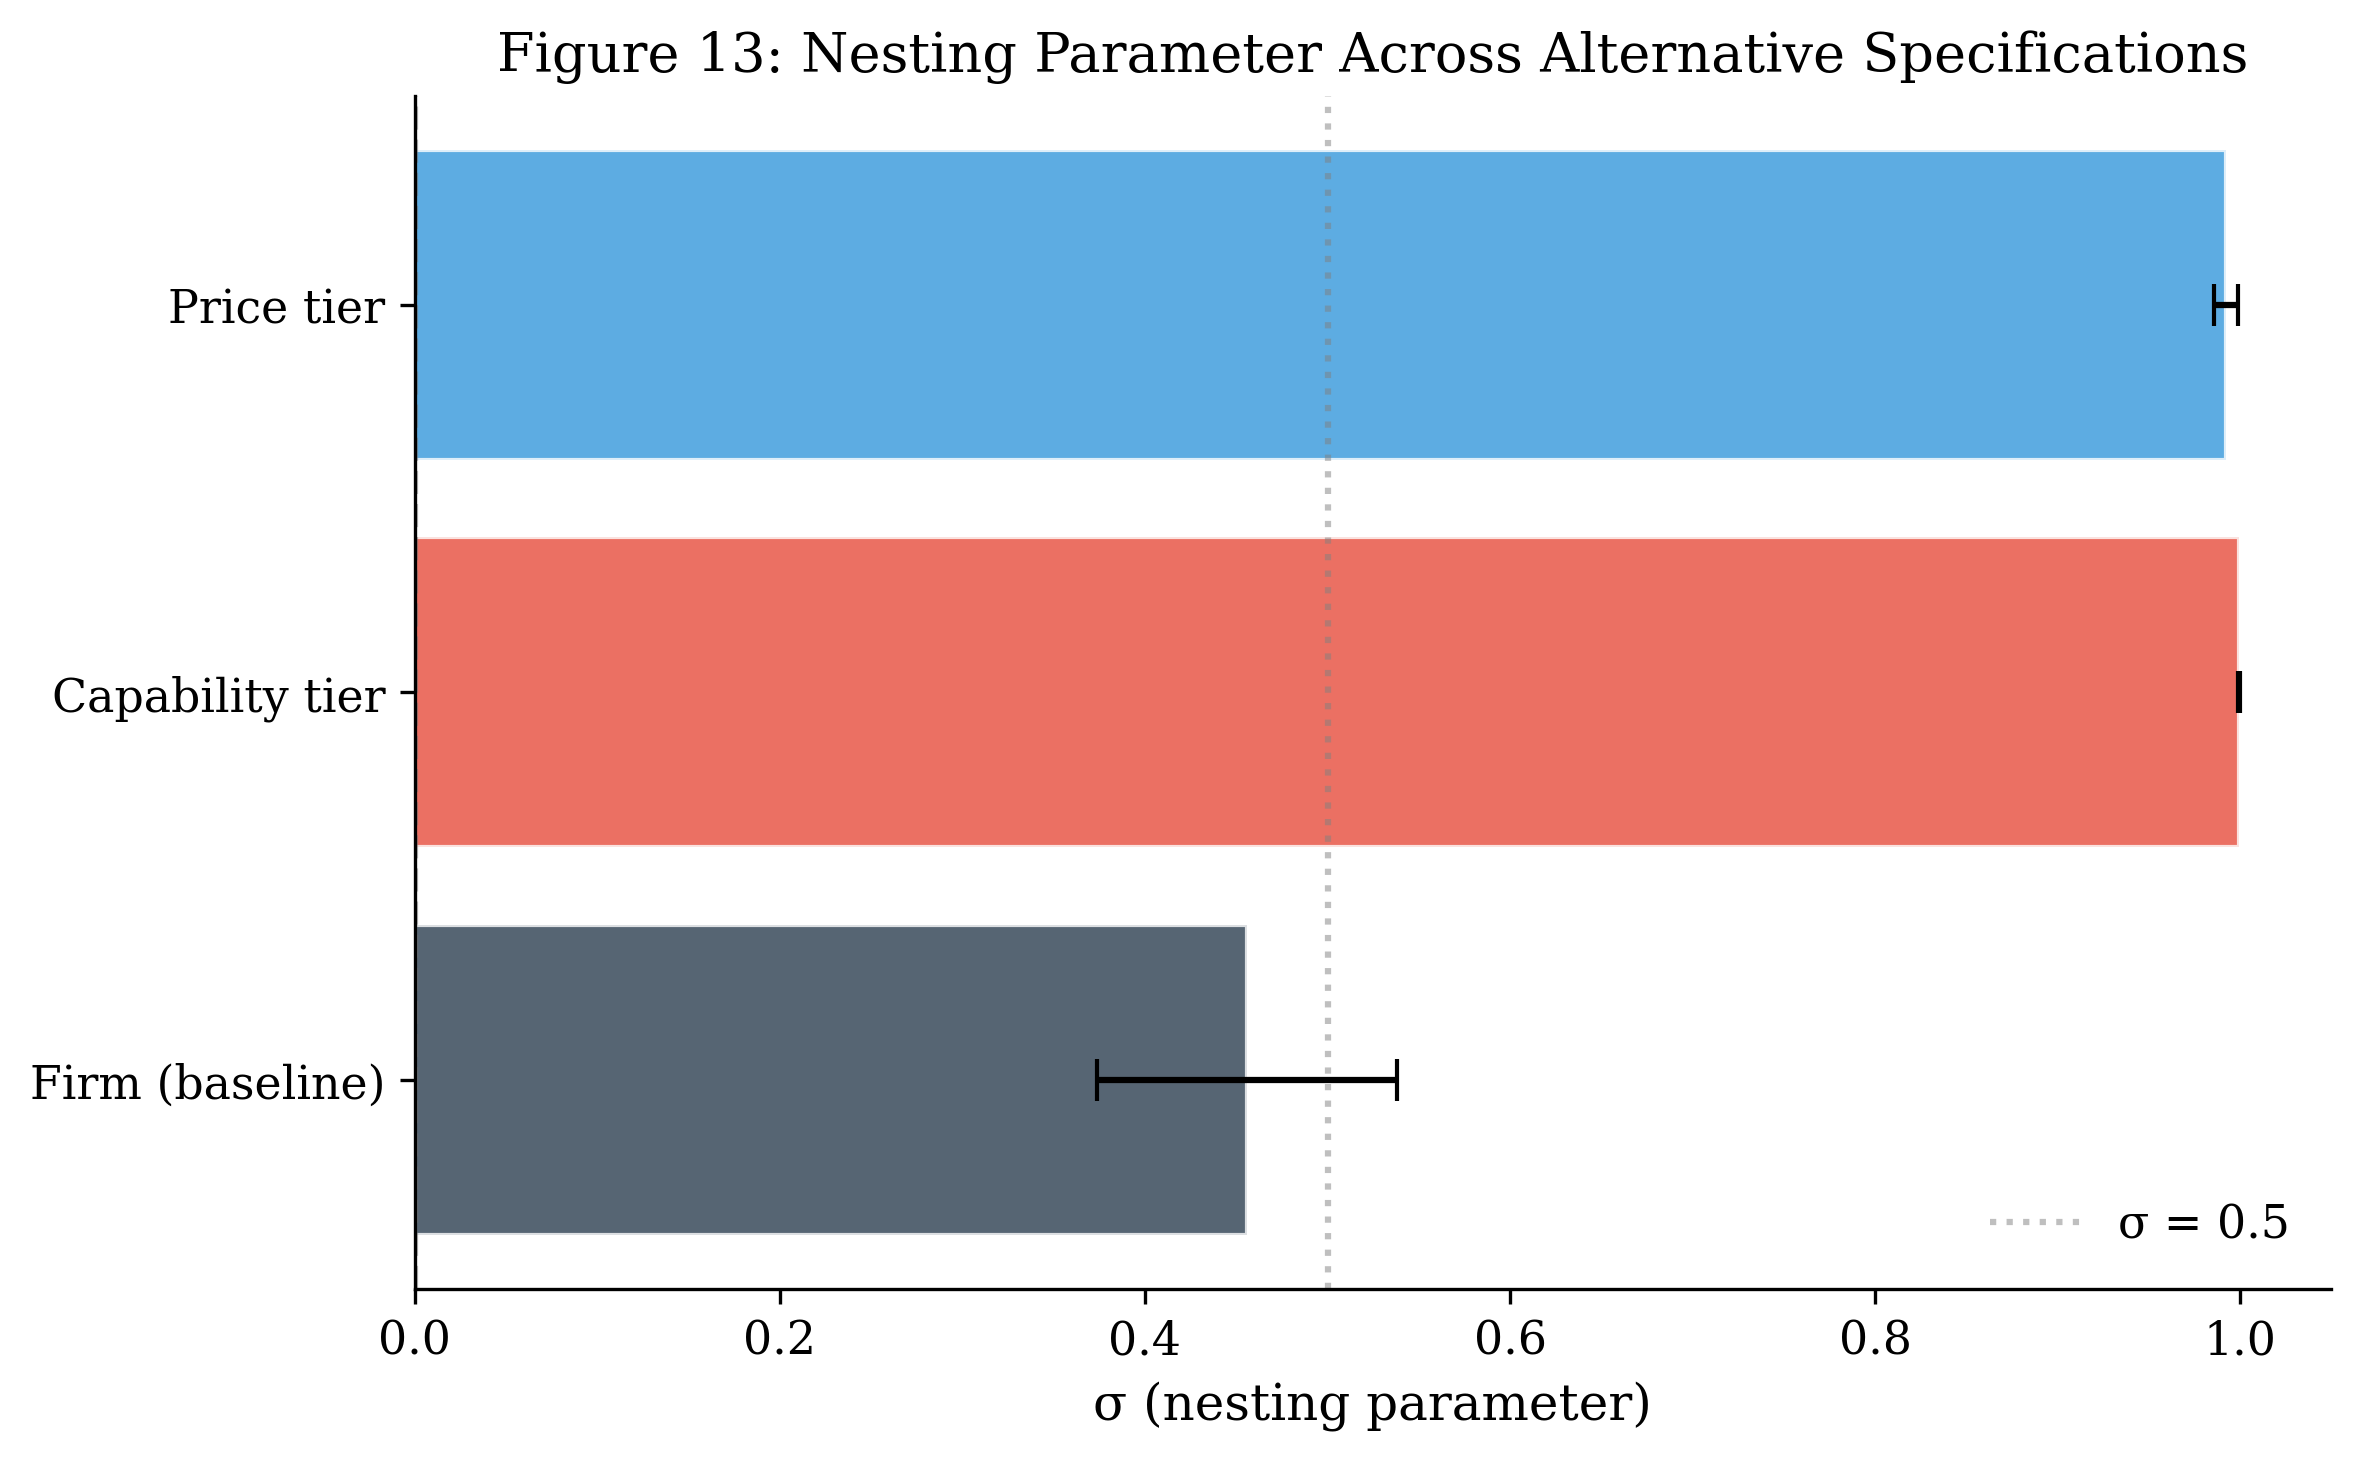
\includegraphics[width=0.85\textwidth]{../output/figures/fig13_robustness_sigma.png}
\caption{Sensitivity of Nesting Parameter to Specification}
\label{fig:sigma_robust}
\par\noindent\small \textit{Notes}: Estimated nesting parameter $\hat{\sigma}$ under alternative specifications: baseline firm-based nesting, reasoning-only subsample, non-reasoning subsample, capability-tier nesting, and price-tier nesting. Error bars show 95\% confidence intervals.
\end{figure}

\begin{figure}[H]
\centering
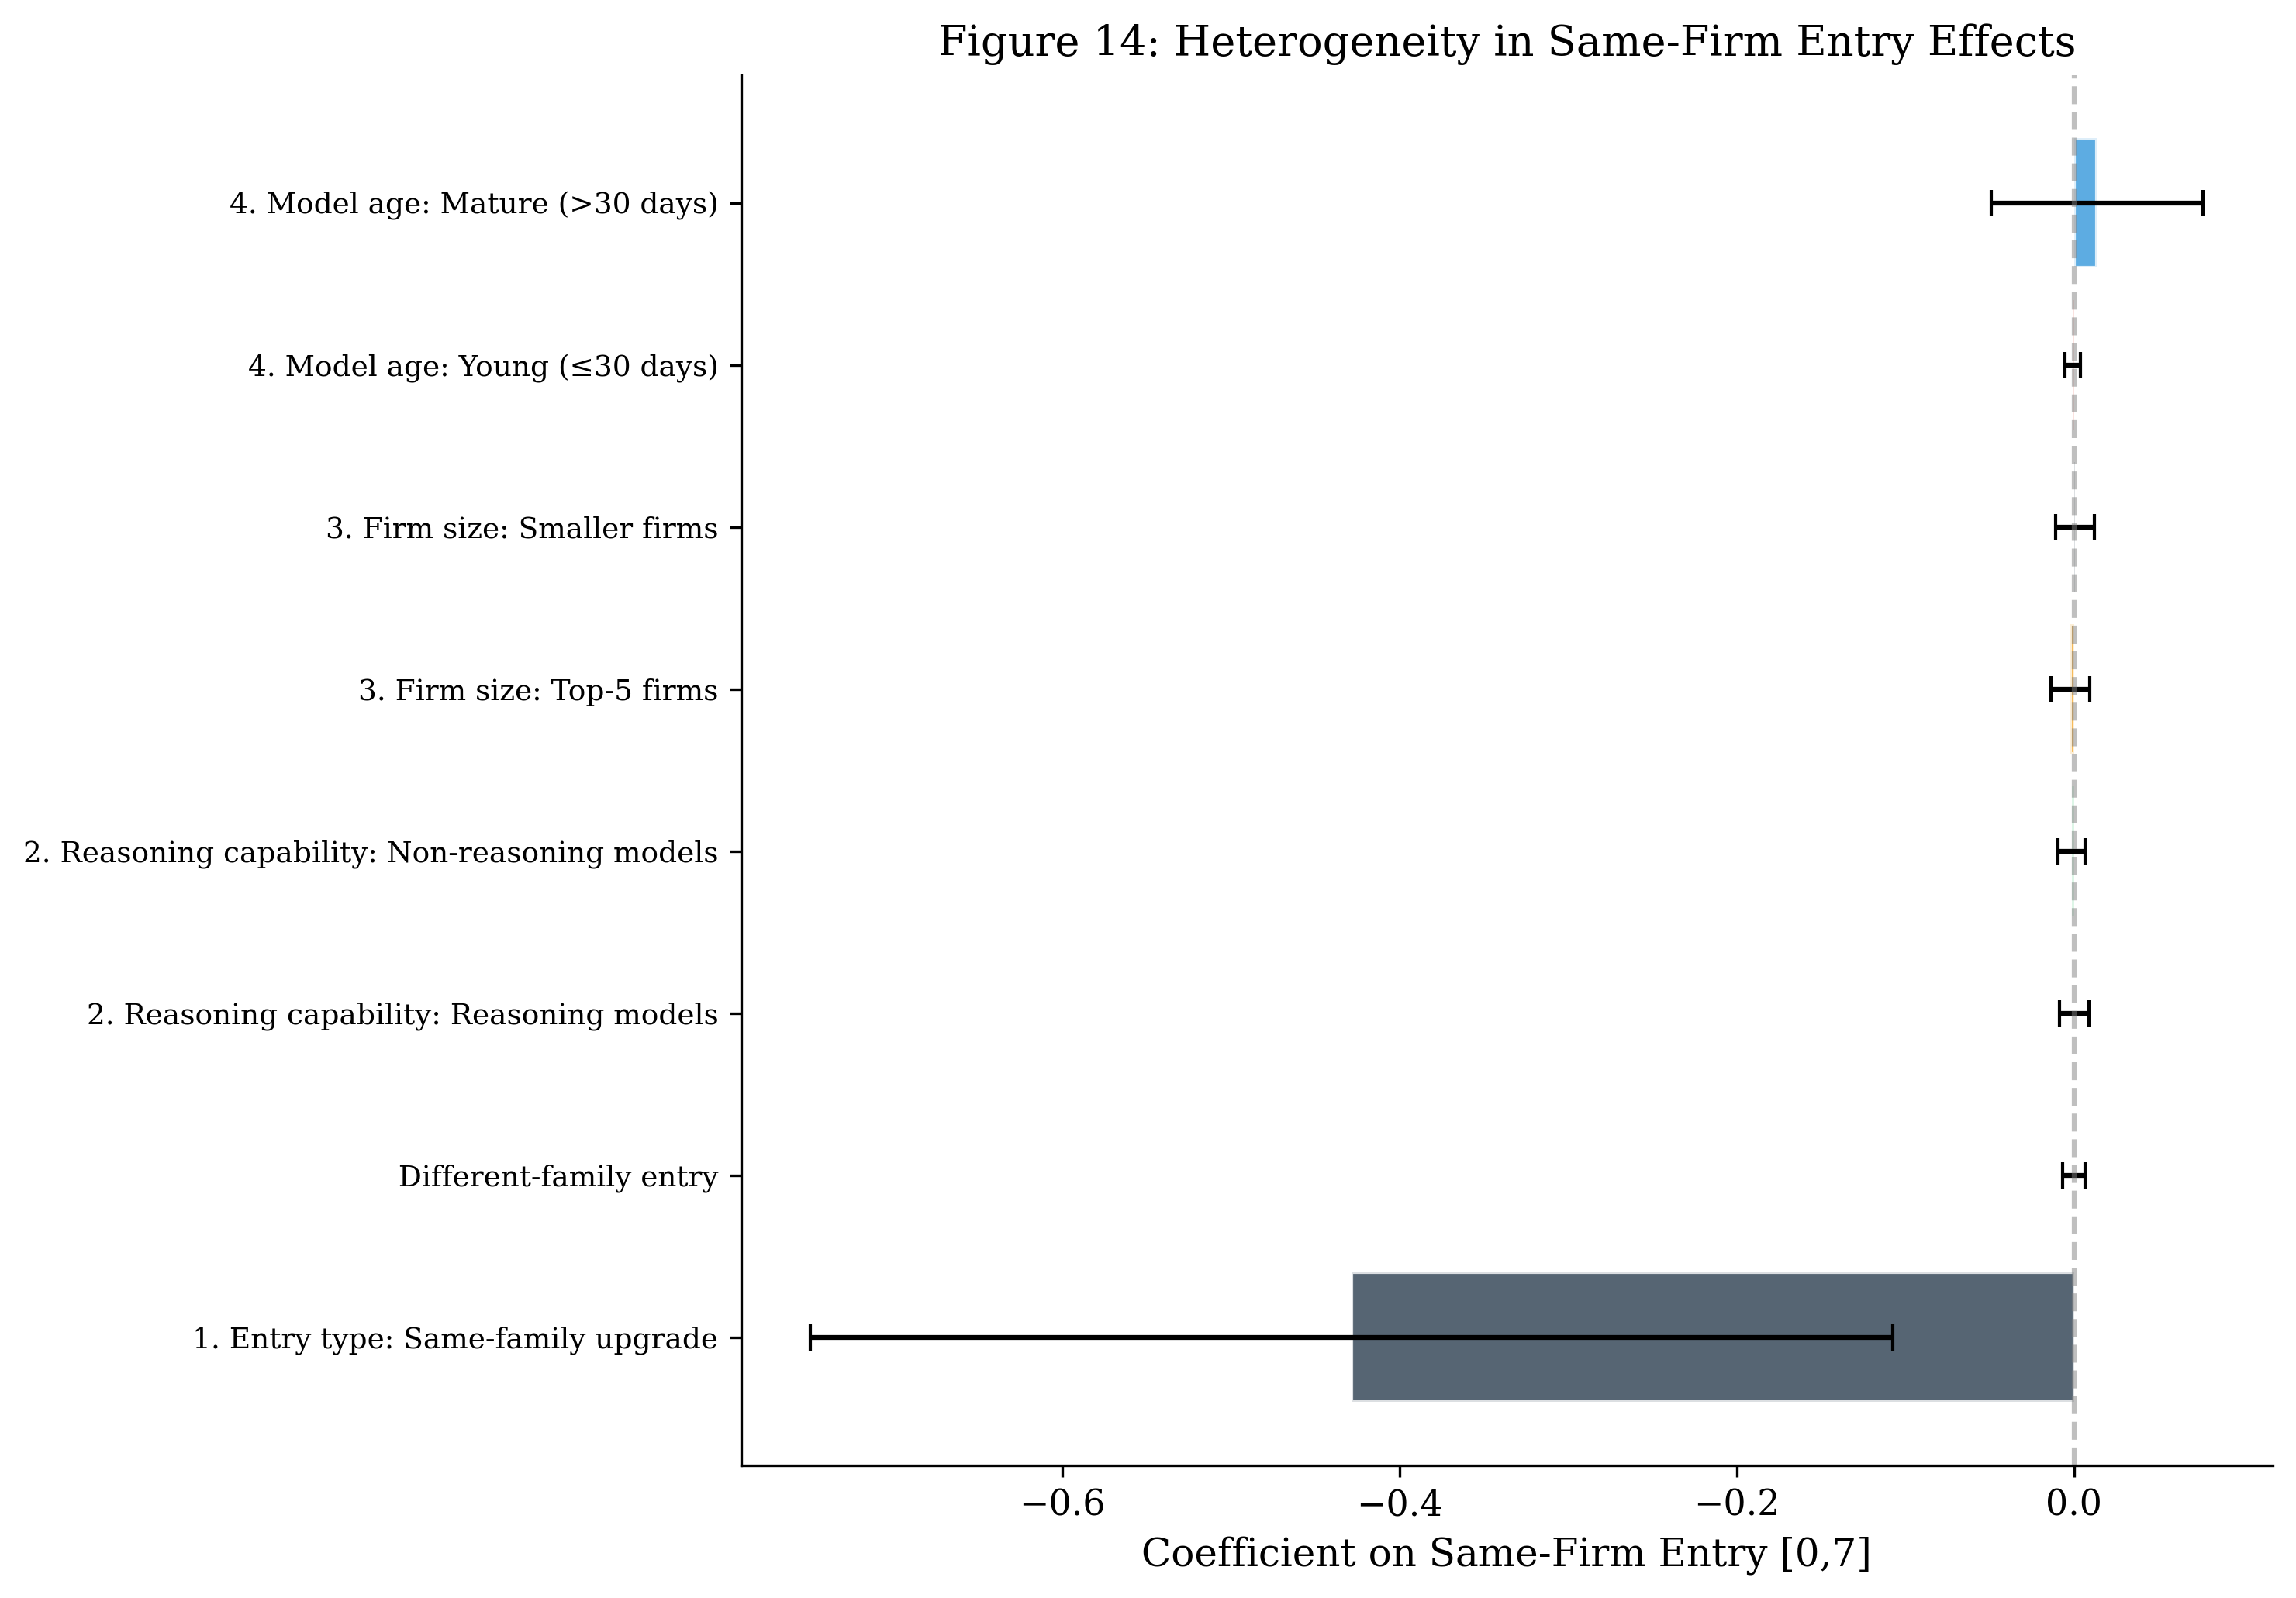
\includegraphics[width=0.85\textwidth]{../output/figures/fig14_heterogeneity.png}
\caption{Heterogeneity in Same-Firm Entry Effects}
\label{fig:het}
\par\noindent\small \textit{Notes}: Same-firm entry $[0,7]$ coefficient estimated separately by subgroup. Error bars show 95\% confidence intervals. The same-family upgrade effect ($-0.43$) is the only statistically significant displacement channel.
\end{figure}

\section{Additional Tables}

\begin{table}[H]
\centering
\caption{Leave-One-Firm-Out Sensitivity}
\label{tab:lofo}
\begin{threeparttable}
\begin{tabular}{lrrr}
\toprule
Excluded firm & $\hat{\beta}$ & SE & $N$ \\
\midrule
Google & $-0.000$ & (0.003) & 28,813 \\
OpenAI & $-0.005$ & (0.005) & 25,514 \\
Mistral & $0.001$ & (0.003) & 28,010 \\
Minimax & $-0.000$ & (0.003) & 30,399 \\
DeepSeek & $-0.001$ & (0.003) & 29,834 \\
\bottomrule
\end{tabular}
\begin{tablenotes}[flushleft]
\small
\item \textit{Notes}: Same-firm entry $[0,7]$ coefficient from equation~\eqref{eq:panel}, re-estimated after excluding all models from the named firm. Model and day fixed effects included. Standard errors clustered at the model level.
\end{tablenotes}
\end{threeparttable}
\end{table}

\section{Data Cleaning and Sample Construction Details}

The raw daily usage panel contains 29,407 rows. We apply the following cleaning steps:
\begin{enumerate}[nosep]
\item Remove duplicate model--date entries (323 rows removed).
\item Exclude the most recent calendar day's data, which may be incomplete due to the platform's retroactive update process.
\item Merge model metadata (firm identity, characteristics, pricing) using model identifiers.
\item Compute derived variables: market shares, within-firm shares, entry indicators, model age.
\item For the nested logit sample, restrict to observations where the outside option share is positive and the within-firm share is well-defined (model appears on a day when at least one other same-firm model also appears). This yields $N = 26{,}444$.
\item For the panel regression sample, retain all models with at least 1,000 total requests. This yields $N = 30{,}903$.
\end{enumerate}

All data cleaning decisions were specified in the pre-analysis plan before estimation. One deviation from the plan: the \texttt{model\_age} variable was dropped from panel specifications with model and day fixed effects, as it is perfectly collinear with the interaction of model identity and calendar date. We retain it in the nested logit specification, which does not include model fixed effects.

\section{Pre-Analysis Plan Deviations}

We document three deviations from the pre-analysis plan:
\begin{enumerate}[nosep]
\item \textbf{Model age dropped from panel regressions.} \texttt{model\_age} is a deterministic function of model identity and date, making it collinear with model $\times$ day fixed effects. This was anticipated as a possibility in the plan.
\item \textbf{Rival entry dropped from TWFE specifications.} The rival entry variable varies only by date (all models face the same number of rival entries on a given day), making it collinear with day fixed effects. We instead estimate the rival entry effect using an entity $\times$ week fixed effects specification that allows sufficient variation.
\item \textbf{Same-family vs.\ different-family decomposition added.} This was not pre-specified but is motivated by the economic distinction between vertical upgrades and horizontal diversification. It is our key finding and is robust across specifications.
\end{enumerate}

\end{appendices}

\end{document}
